\documentclass{beamer}

\usepackage{pgfpages}

%\setbeameroption{show only notes}

\setbeamertemplate{section in toc}[sections square]
\setbeamertemplate{subsection in toc}[subsections square]

\setbeamertemplate{section in toc}{%
    \usebeamercolor[fg]{enumerate item}%
    \makebox[1em][l]{\color{JGURed}\scriptsize$\blacksquare$}%
    \parbox[t]{\dimexpr\linewidth-2em}{\inserttocsection}%
}

\setbeamertemplate{subsection in toc}{%
    \usebeamercolor[fg]{enumerate item}%
    \makebox[1.5em][l]{}%
    \makebox[1em][l]{\color{JGURed}\scriptsize$\blacktriangleright$}%
    \parbox[t]{\dimexpr\linewidth-2em}{\inserttocsubsection}%
    %\vspace{2mm}
}

\setbeamertemplate{bibliography item}[text]

\AtBeginSection[]{%
  \begin{frame}[plain,c]
    \centering
    \vspace*{1.8cm}
    %\hspace*{0.5cm}
    \textcolor{JGURed}{\huge{\insertsection}}
  \end{frame}
  \addtocounter{framenumber}{-1}% If you don't want them to affect the slide number
}

\AtBeginSubsection[]{%
  \begin{frame}[plain,c]
    \centering
    \vspace*{1.5cm}
    %\hspace*{0.5cm}
    \textcolor{JGUGrau}{\insertsection}\\
    \vspace*{0.2cm}
    \textcolor{JGURed}{\huge{\insertsubsection}}
  \end{frame}
  \addtocounter{framenumber}{-1}% If you don't want them to affect the slide number
}


\usepackage{helvet}
\usepackage{hyperref}
\usepackage{amsmath, amssymb}
\usepackage[utf8]{inputenc}
\usepackage{graphicx}
\usepackage{multirow}
\usepackage{url}
\usepackage{siunitx}
\sisetup{
separate-uncertainty = true
}
\usepackage{color}
\usepackage{bookmark}
\usepackage[]{placeins}
\usepackage{tikz}
\usetikzlibrary{calc,shapes,arrows}
\usepackage{listings}
\usepackage{anyfontsize}

\usepackage[
    backend=biber,
    %style=authoryear-icomp,
    % sortlocale=de_DE,
    % natbib=true,
    % url=false,
    % doi=true,
    % eprint=false
]{biblatex}
\addbibresource{sources.bib}
\renewcommand*{\bibfont}{\tiny}

\usepackage{hyperref}
\usepackage{geometry}
\geometry{
  left=3.0cm,
  right=0.0cm,
  bottom=7mm,
  top=0mm
}
\unitlength = 1mm

\renewcommand{\familydefault}{\sfdefault}


\setbeamertemplate{frametitle}{\vspace*{0.3cm}\insertframetitle\\}
\setbeamersize{text margin left=10pt}
\setbeamertemplate{navigation symbols}{}

\definecolor{JGURed}{RGB}{193,0,42}
\definecolor{JGUGrau}{RGB}{99,99,99}
\definecolor{JGULight}{RGB}{172,172,172 }
%\setbeamertemplate{items}{\textcolor{JGURed}$\textbullet$}

\setbeamertemplate{itemize item}{\color{JGURed}\scriptsize$\blacksquare$}
\setbeamertemplate{itemize subitem}{\color{JGURed}\scriptsize$\blacktriangleright$}



\setbeamercolor{frametitle}{fg=JGURed}
\setbeamercolor{title}{fg=JGURed}
\setbeamercolor{subtitle}{fg=JGURed}
\setbeamercolor{author}{fg=JGUGrau}
\setbeamercolor{institute}{fg=JGUGrau}
\setbeamercolor{date}{fg=JGUGrau}
\setbeamercolor{navigation symbols}{fg=JGUGrau}


\title{Development of TRatioPlot in ROOT}
\subtitle{SFT Group  Meeting}
\author{Paul Gessinger}
\institute{Johannes Gutenberg University Mainz  \\ \vspace*{.3cm}\tiny{Supervisors:} \\ \small Olivier Couet \\ Lorenzo Moneta }
\date{19.09.2016}

\setbeamercolor{structure}{fg=black}
\setbeamercolor{normal text}{fg=black}



\setbeamertemplate{footline}{

    \begin{flushright}
      \textcolor{JGUGrau}{SFT Group  Meeting - 19.09.2016}
      \hspace{4.5cm}
      \textcolor{JGUGrau}{\insertframenumber{}} \hspace*{1mm} \\
    \end{flushright}
    %\vspace*{-3mm}
}

\begin{document}
  \newgeometry{
   left=0.8cm,
   right=0.8cm,
   bottom=7mm,
   top=0mm
  }

\begin{frame}
 	\titlepage
\end{frame}


\begin{frame}{}

   %\vspace*{-0.8cm}
   \begin{columns}
    \hspace*{-1.75cm}
    \column{0.7\textwidth}
      \centering
      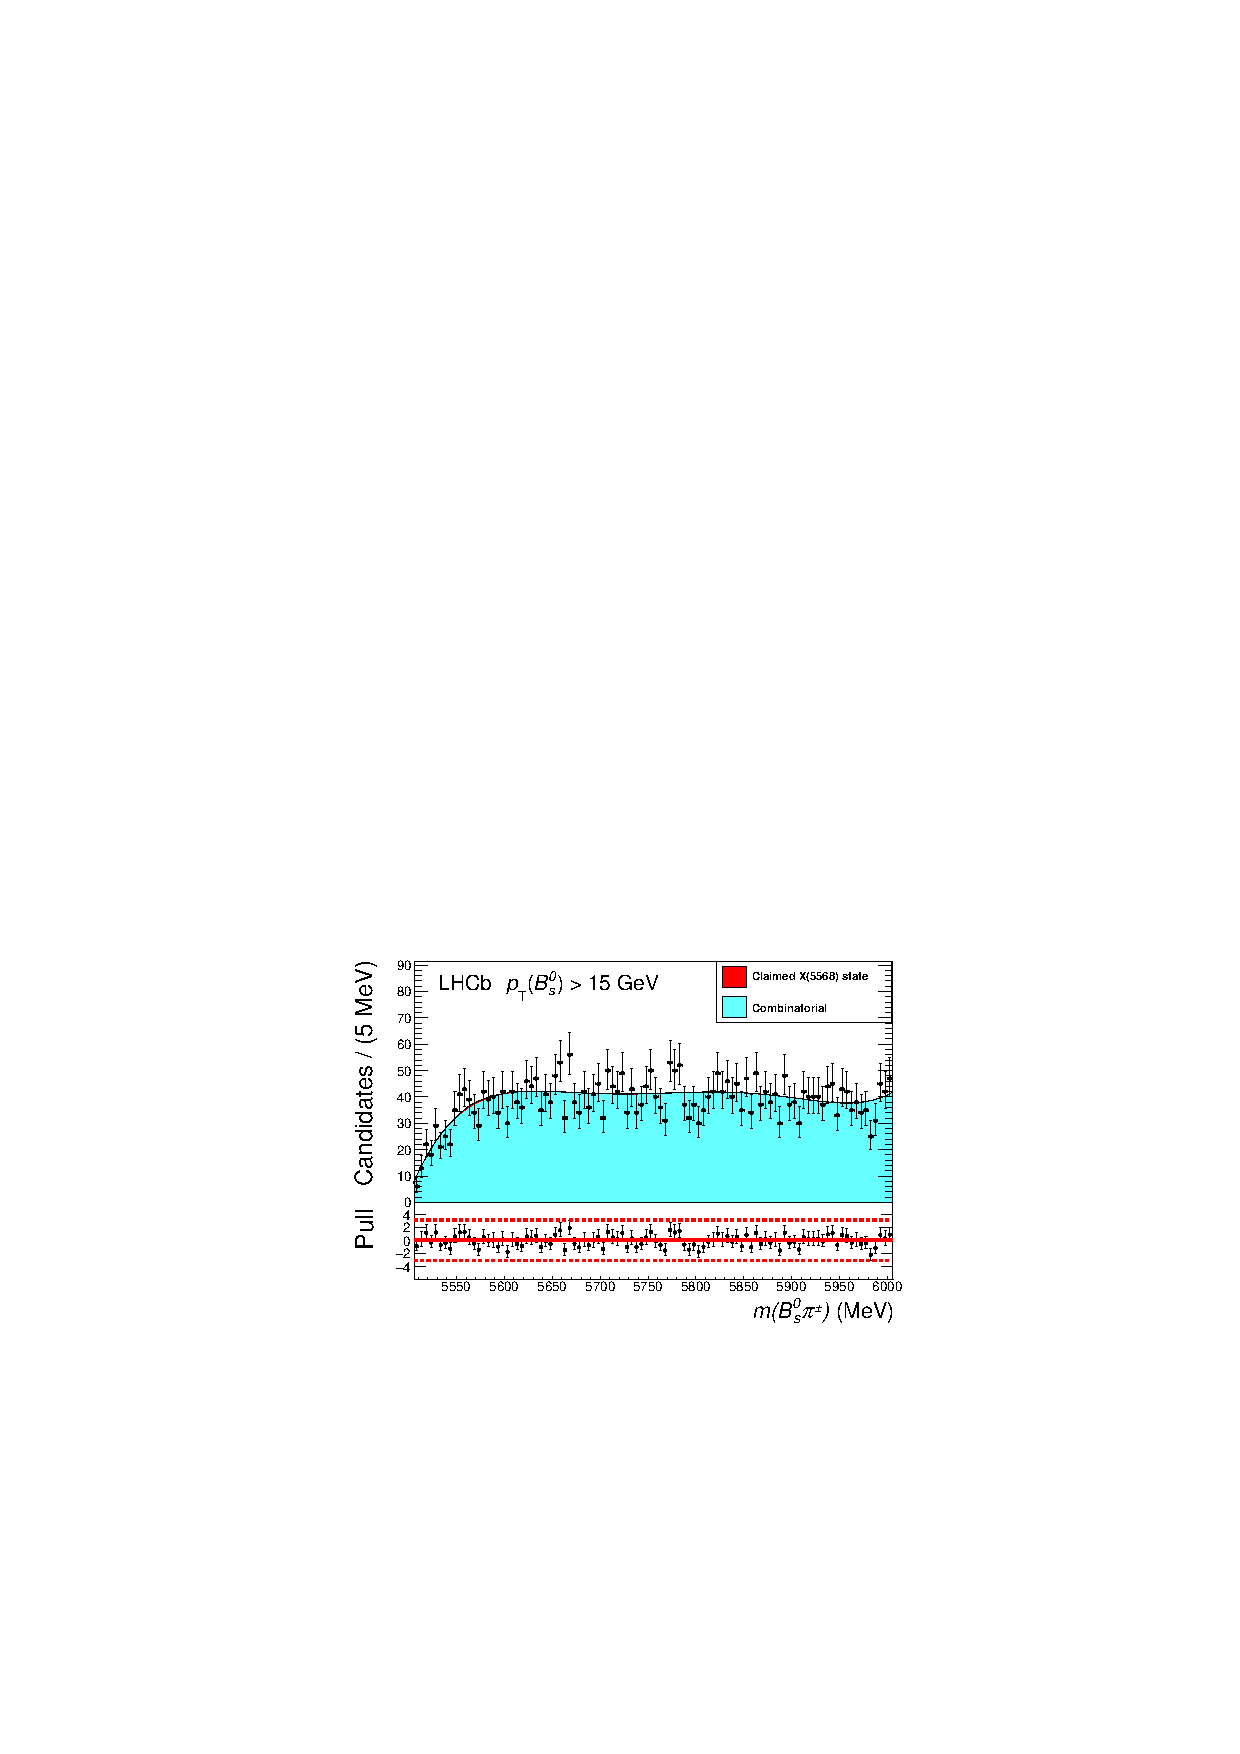
\includegraphics[width=0.65\textwidth]{assets/lhcb_ratio.pdf}
      \vspace*{-0.2cm}
      \tiny{\cite{Aaij:2016iev}} \\
      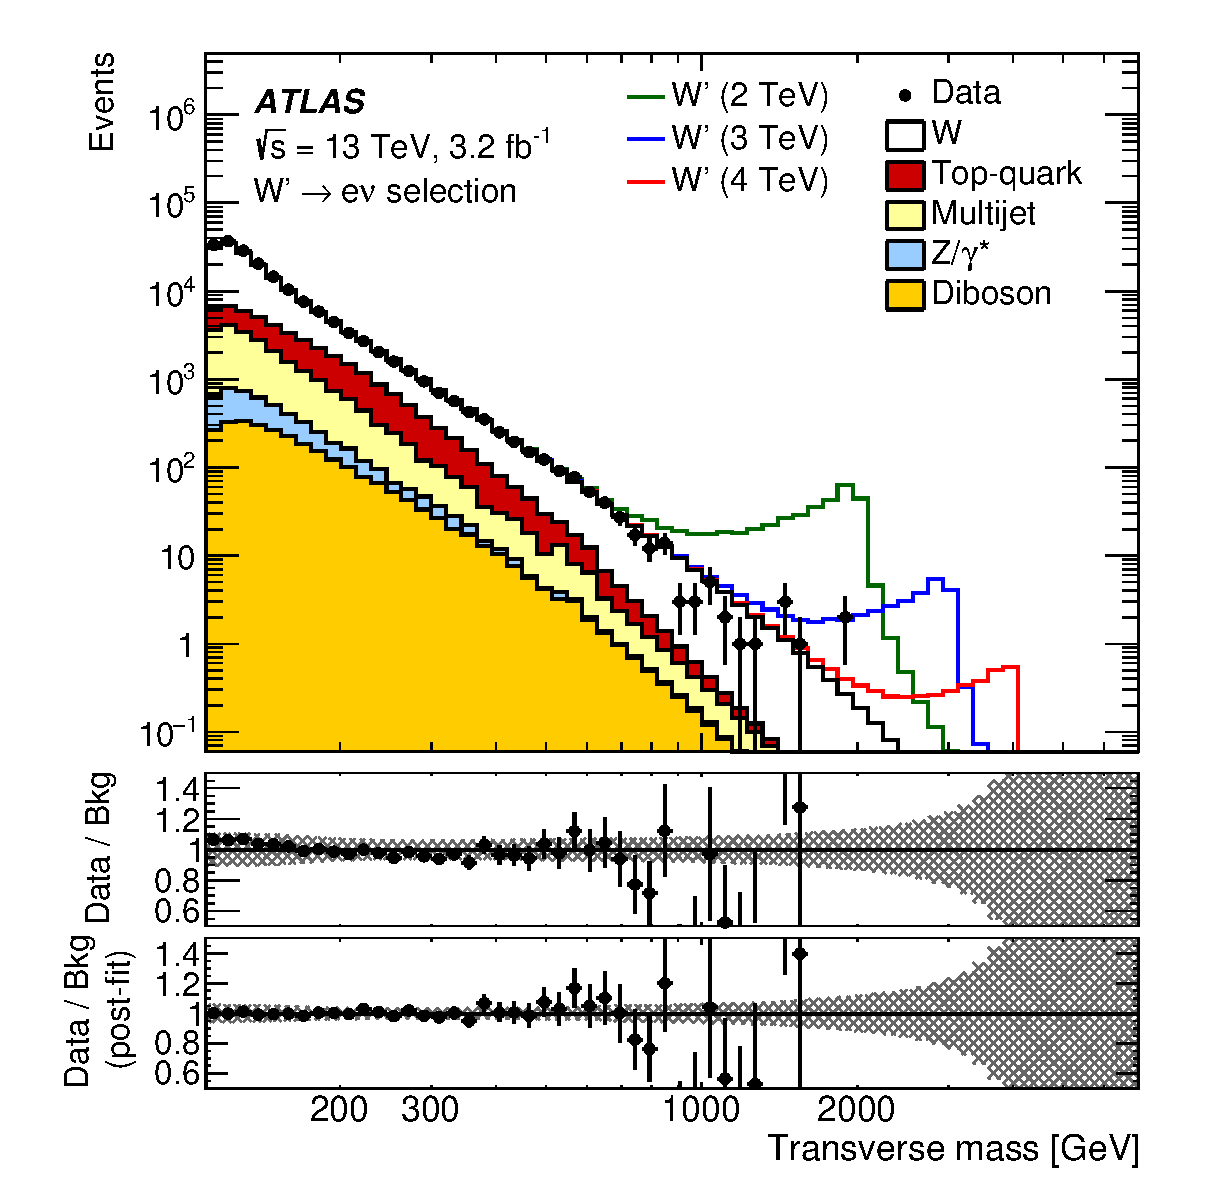
\includegraphics[width=0.6\textwidth]{assets/lmet.eps}
      \tiny{\cite{Aaboud:2016zkn}}
    \column{0.5\textwidth}
      \hspace*{-1cm}
      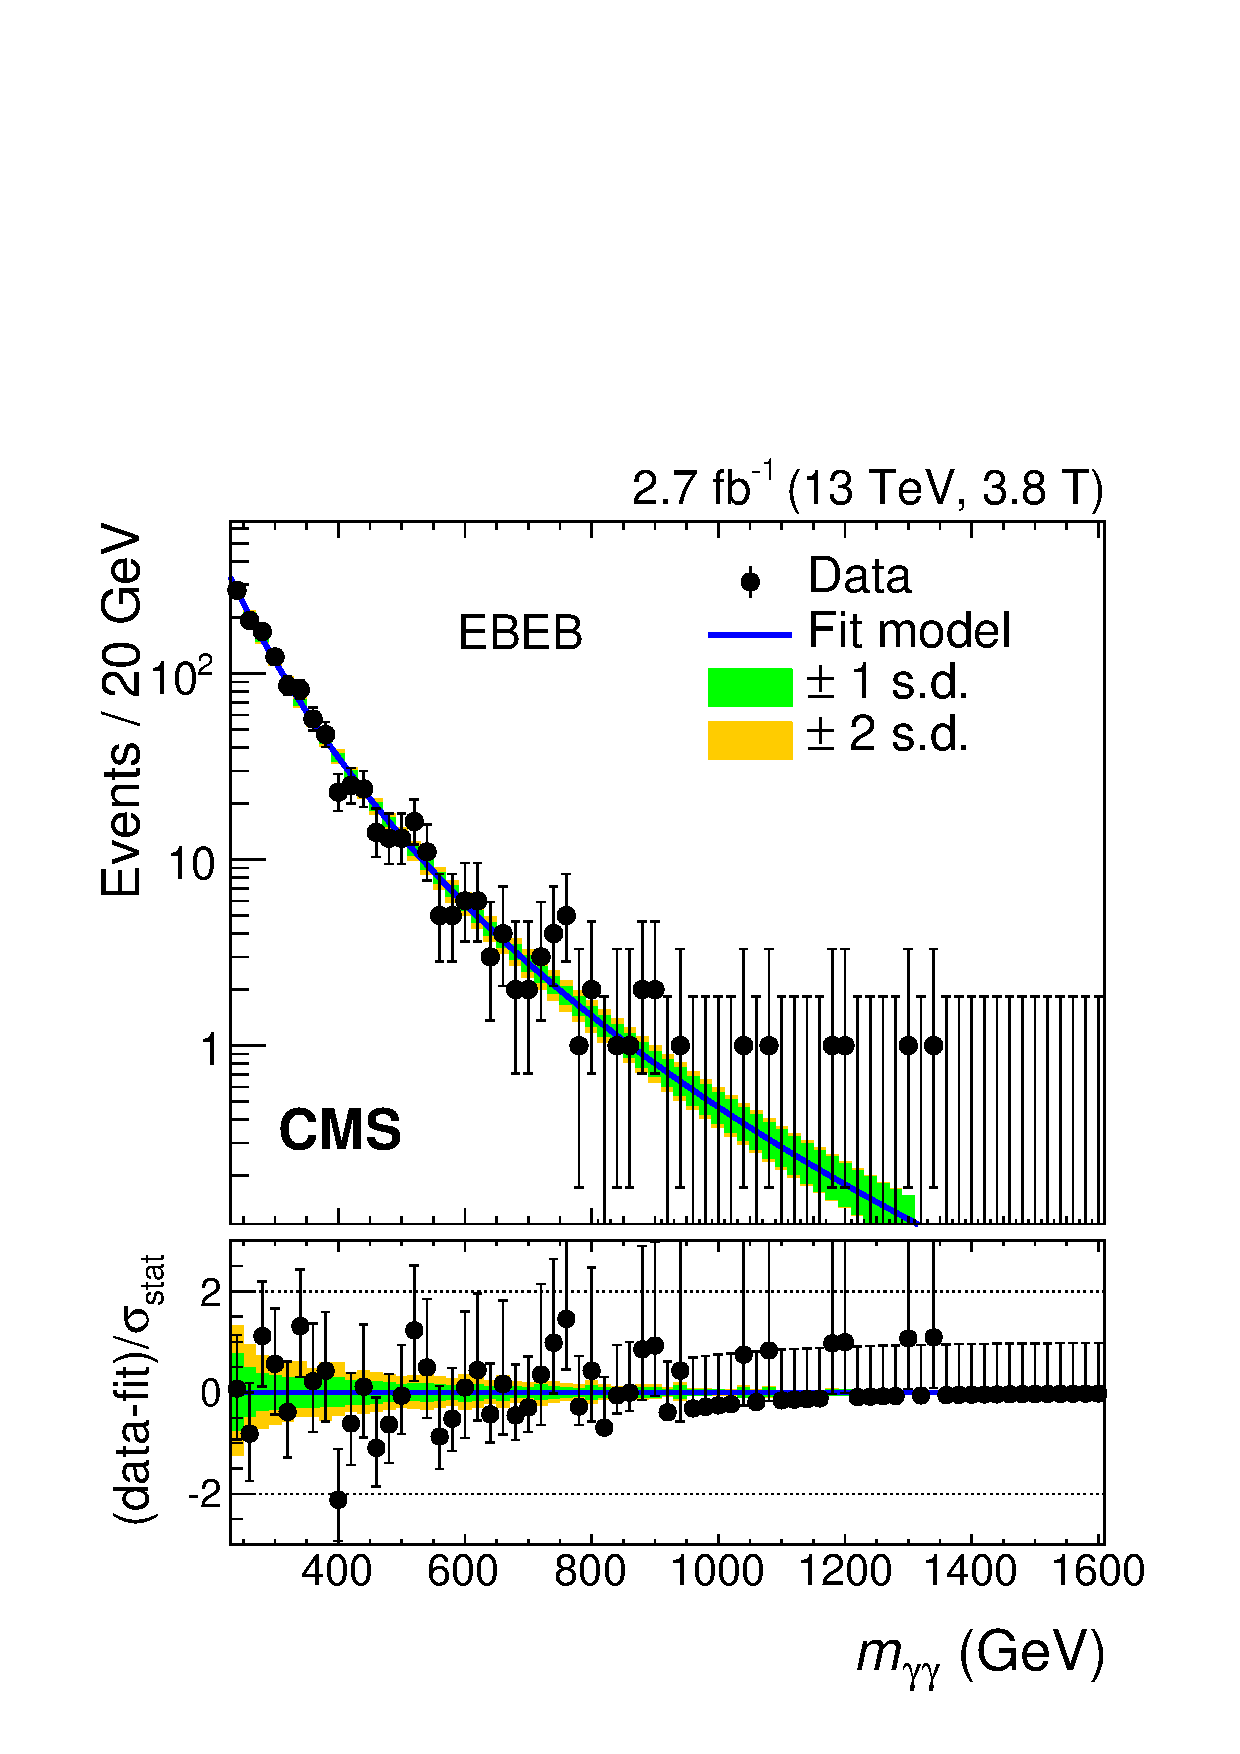
\includegraphics[width=1\textwidth]{assets/diphoton_cms.pdf} \\
      \tiny{\cite{Khachatryan:2016hje}}
  \end{columns}
\end{frame}

\begin{frame}{Existing facilities}
  \only<1>{
  \begin{itemize}
    \item Pads can be subdivided into subpads
    \item All of the same size
    \item Manually create pads and align them
    \begin{itemize}
      \item But: Pads have coordinate system depending on their drawn content
      \item Font sizes are dependent on size of the pad within parent
      \item Axis ranges are independent
    \end{itemize}
  \end{itemize} 
  }
  \only<2>{
  \centering
  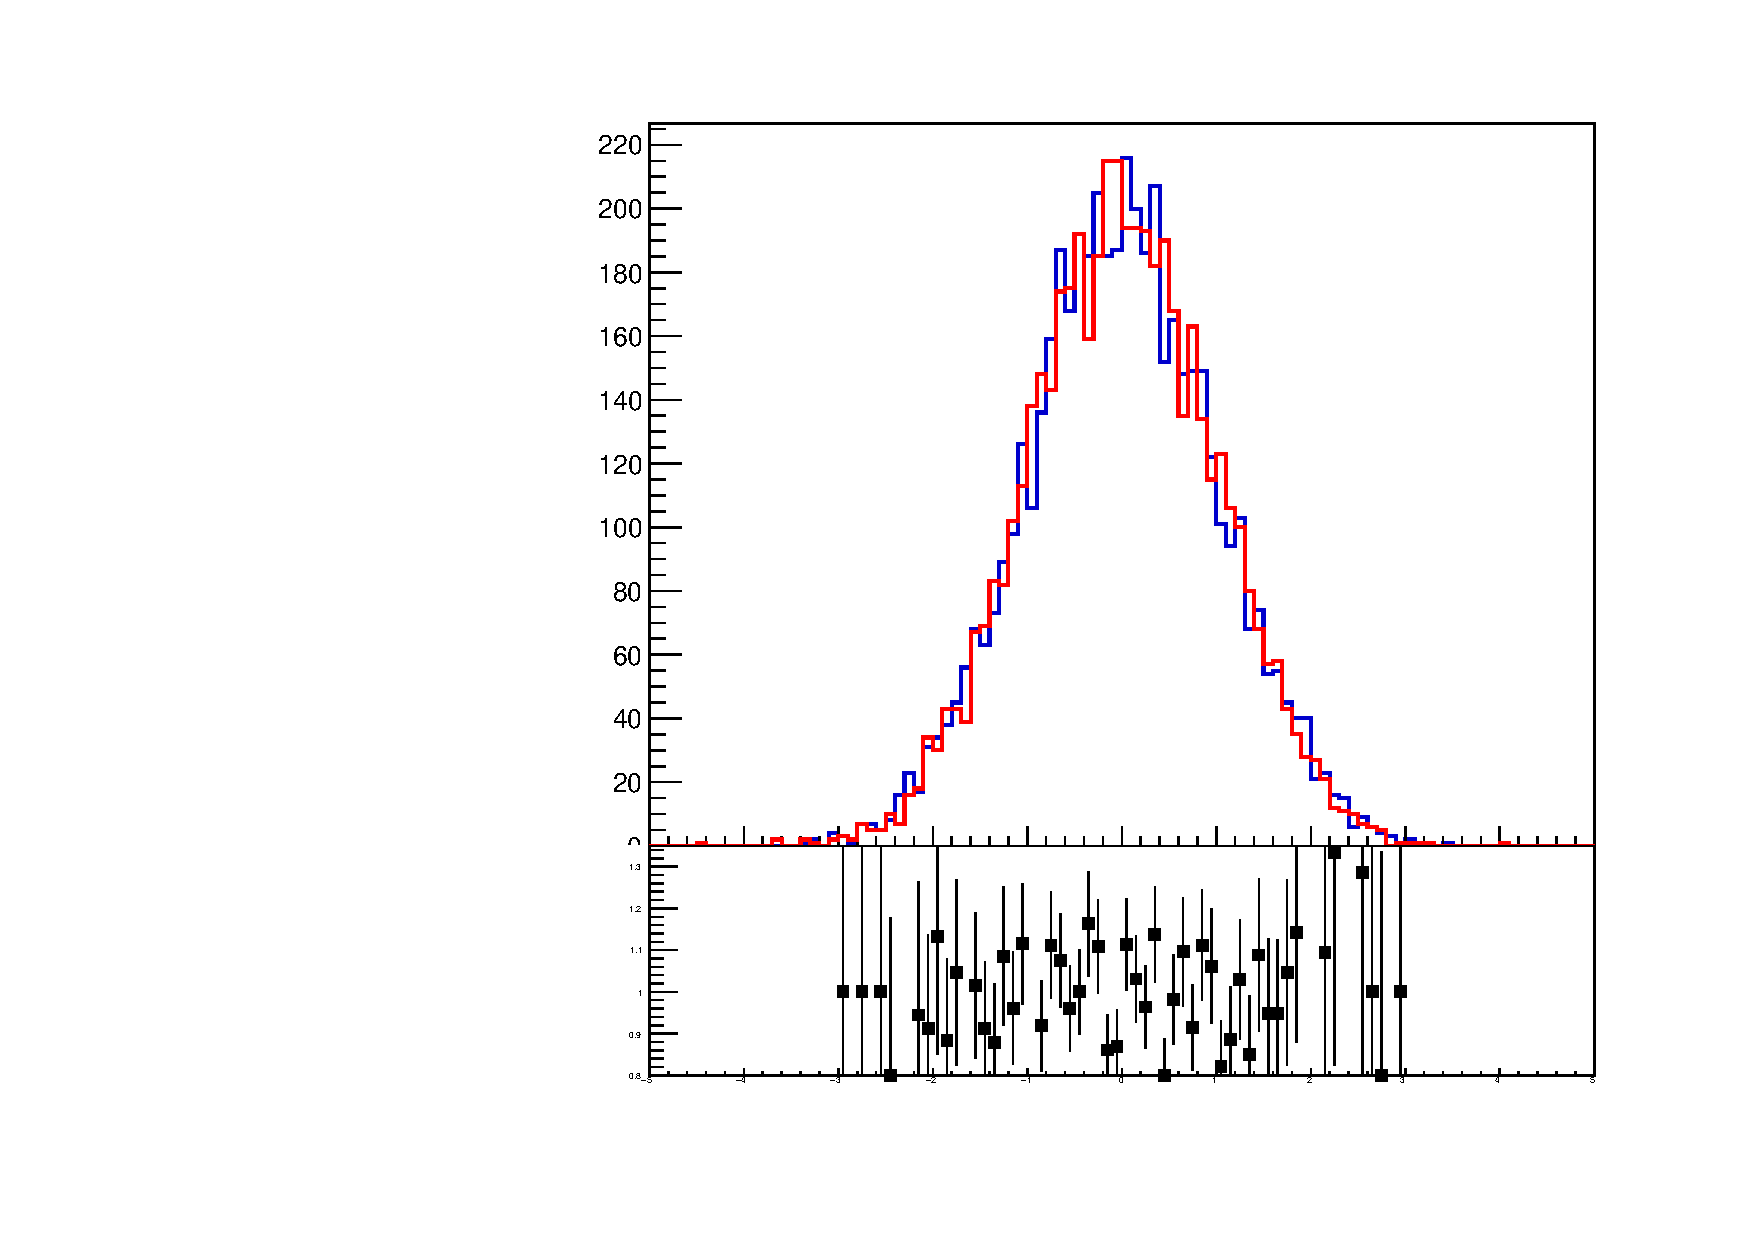
\includegraphics[width=0.8\linewidth]{assets/bad.pdf}
  }
\end{frame}


\begin{frame}[t]{Design goals}
  \begin{itemize}
    \item Make visualization consistent and remove redundancy
    \begin{itemize}
      \item Link two \texttt{TPad}s together
      \item Consistent labels, ticks and tickmarks
    \end{itemize}
    \item Improve interactively working with this type of plot
    \begin{itemize}
      \item Displays should be synchronized automatically
      \item Elements should be customizable through the Editor
    \end{itemize}
    \item Implement most common calculations in the class, and implement usual graphical display
    \begin{itemize}
      \item Ratio of two histograms
      \item Difference between two histograms
      \item Fit residual between a histogram and a fitted function (shows confidence interval bands)
    \end{itemize}
  \end{itemize}  
\end{frame}

\section{Display structure}
\begin{frame}[t]{\insertsection}
  \only<1>{
  \centering
  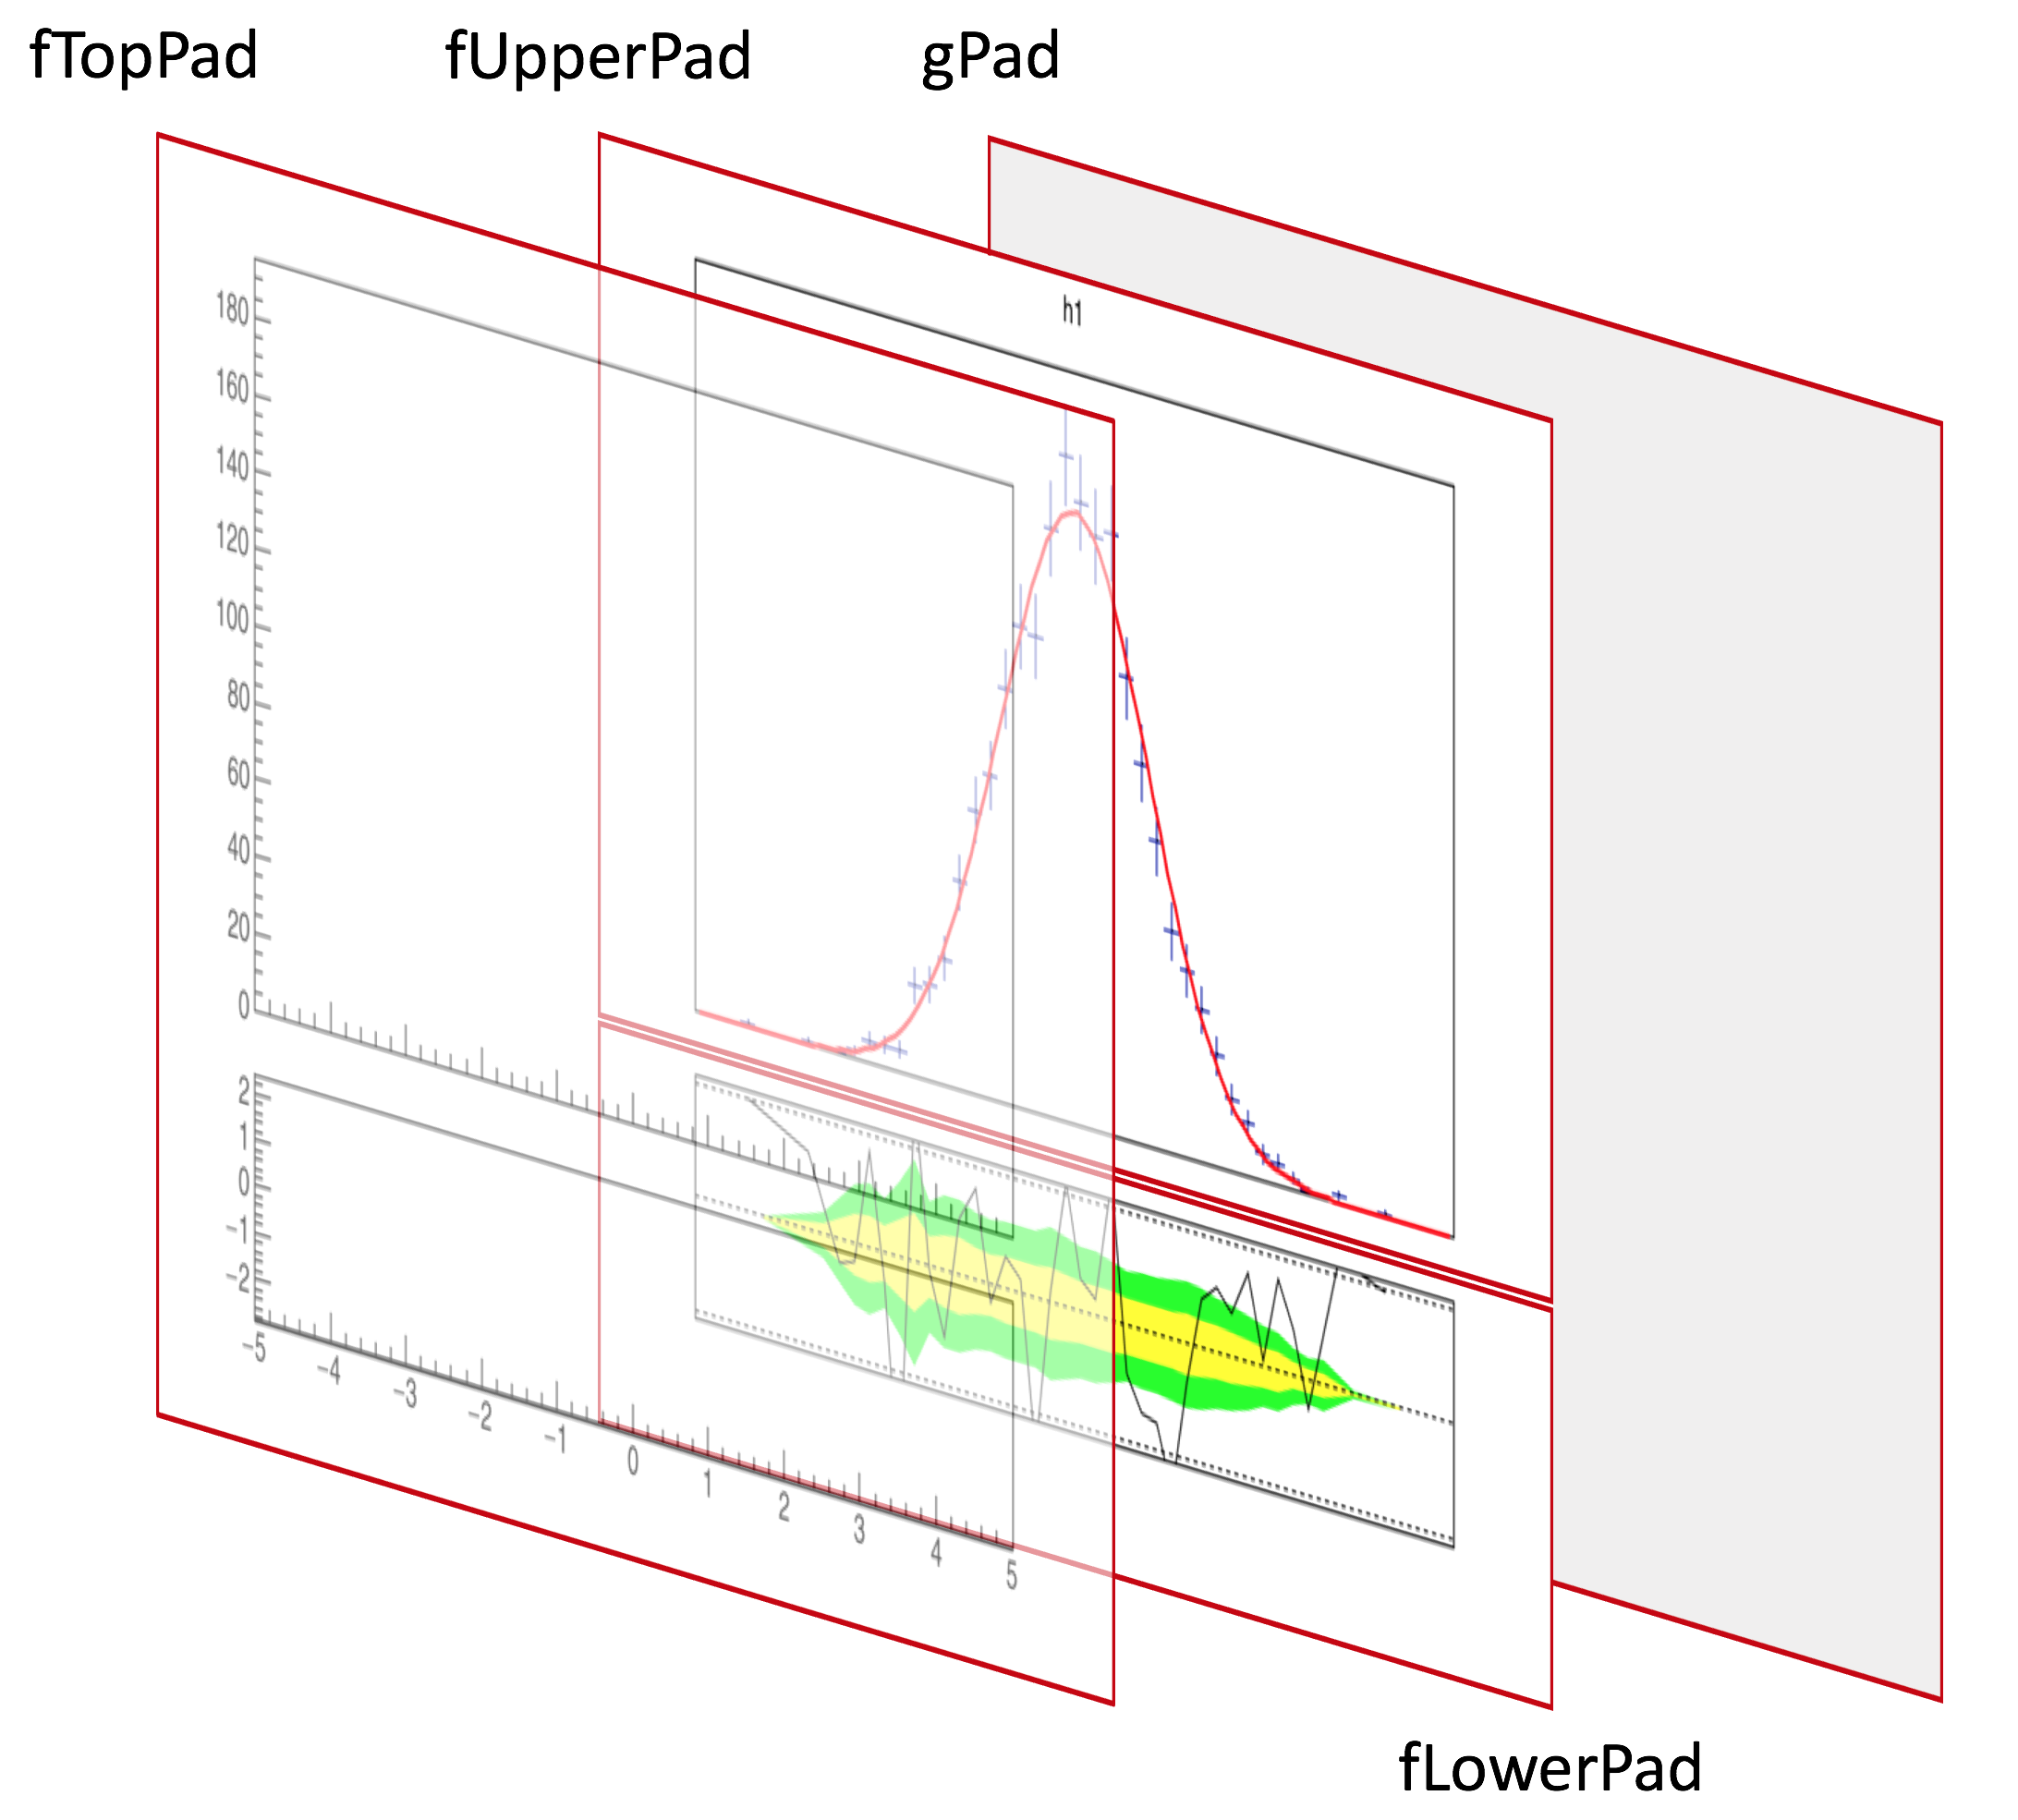
\includegraphics[width=0.7\linewidth]{assets/padstack.png}
  }
  \uncover<2->{
  \begin{columns}
    \column{0.5\linewidth}
    \begin{itemize}
      \item Two pads which contain the input histograms and the calculation output
      \item Additional transparent pad on top, which receives the \texttt{TGAxis}
      \item This pad needs to pass through interaction:
        \begin{itemize}
          \item Modified \texttt{TPad} to not participate in Pick/ExecuteEvent calls when the bit \texttt{kCannotPick} is set
        \end{itemize}
    \end{itemize}
    \column{0.5\linewidth}
    \centering
    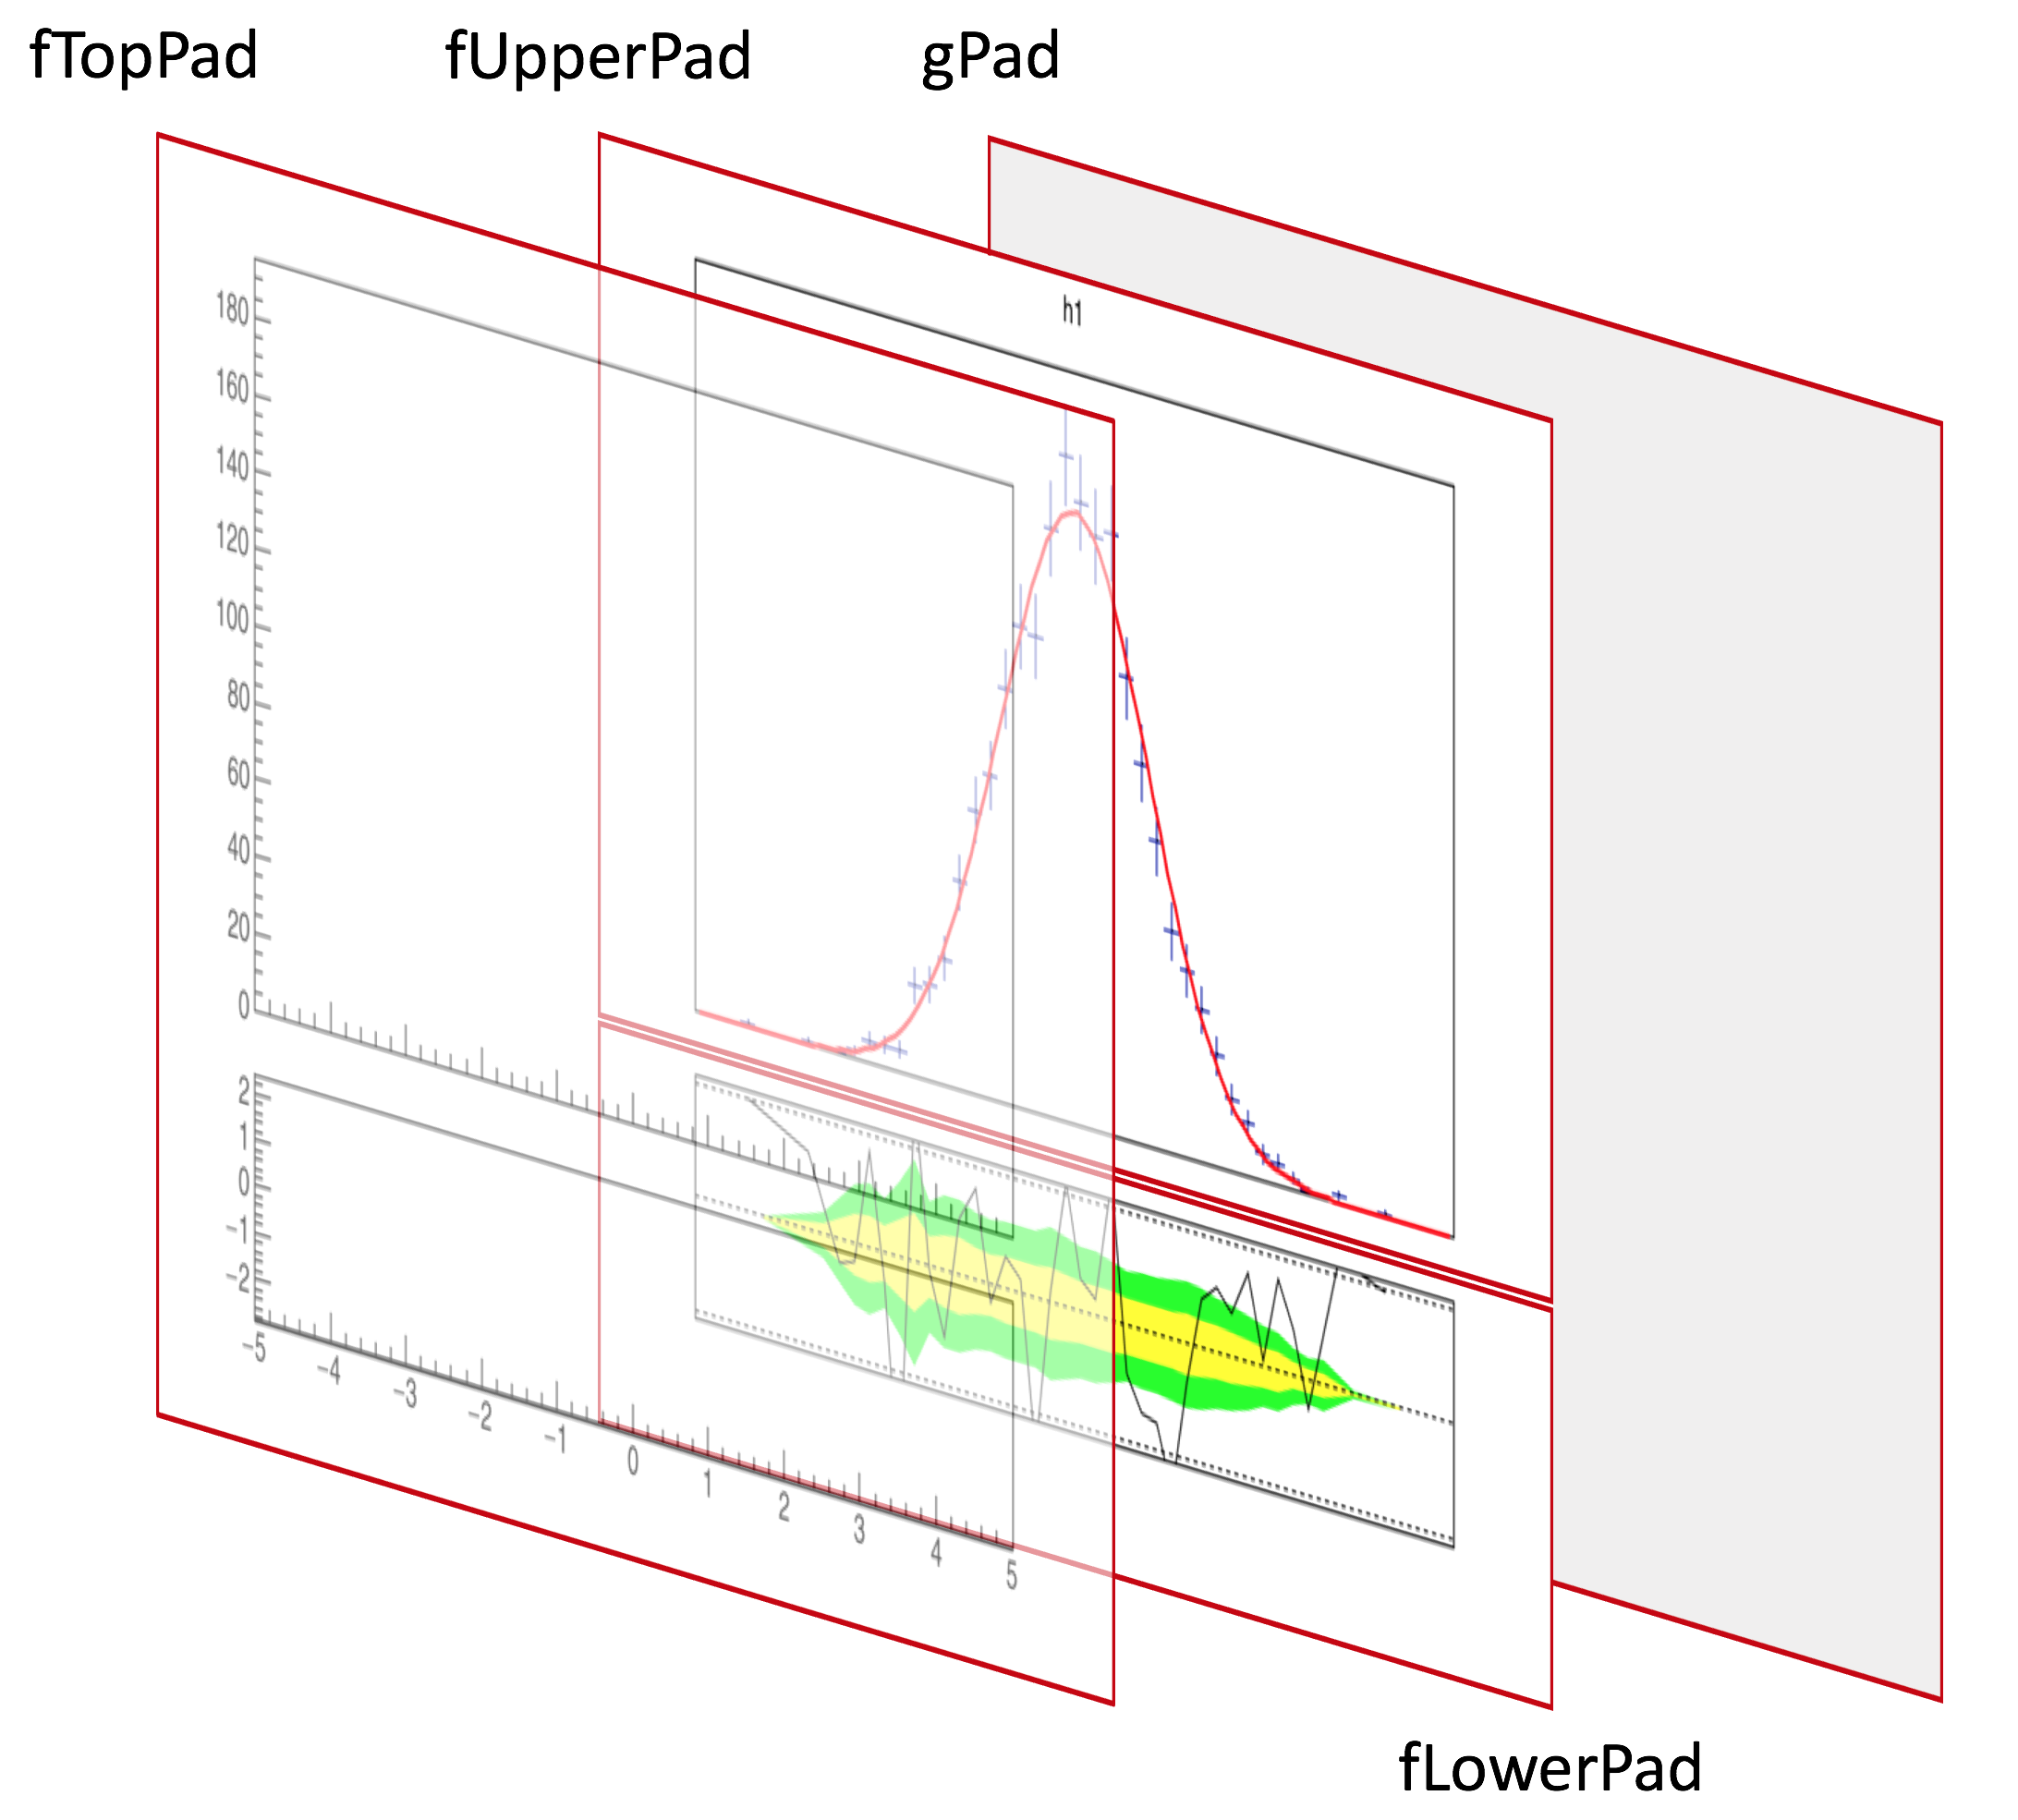
\includegraphics[width=1\linewidth]{assets/padstack.png}  
  \end{columns}
  }
\end{frame}

\begin{frame}[t]{Drawing of graphical elements}
  \begin{itemize}
    \item Original axis drawing is disabled through draw options
    \item Axes are drawn on top pad, so all sizes are consistent
    \item Tick mark sizes depend on the length of the axis, normalization by ratio of pad sizes
  \end{itemize}

  \begin{itemize}
    \item Lower plot can contain dashed lines that are drawn at specified y values
    \item Can alse be disabled with draw option
    \item Useful defaults are set for different modes
  \end{itemize}

  \begin{itemize}
    \item New facility to change axis label attributes
  \end{itemize}
\end{frame}

\begin{frame}[t]{New facility to change axis label attributes}
  \tiny
  \lstinputlisting[language=C++]{assets/tgaxis.C}
  \centering
	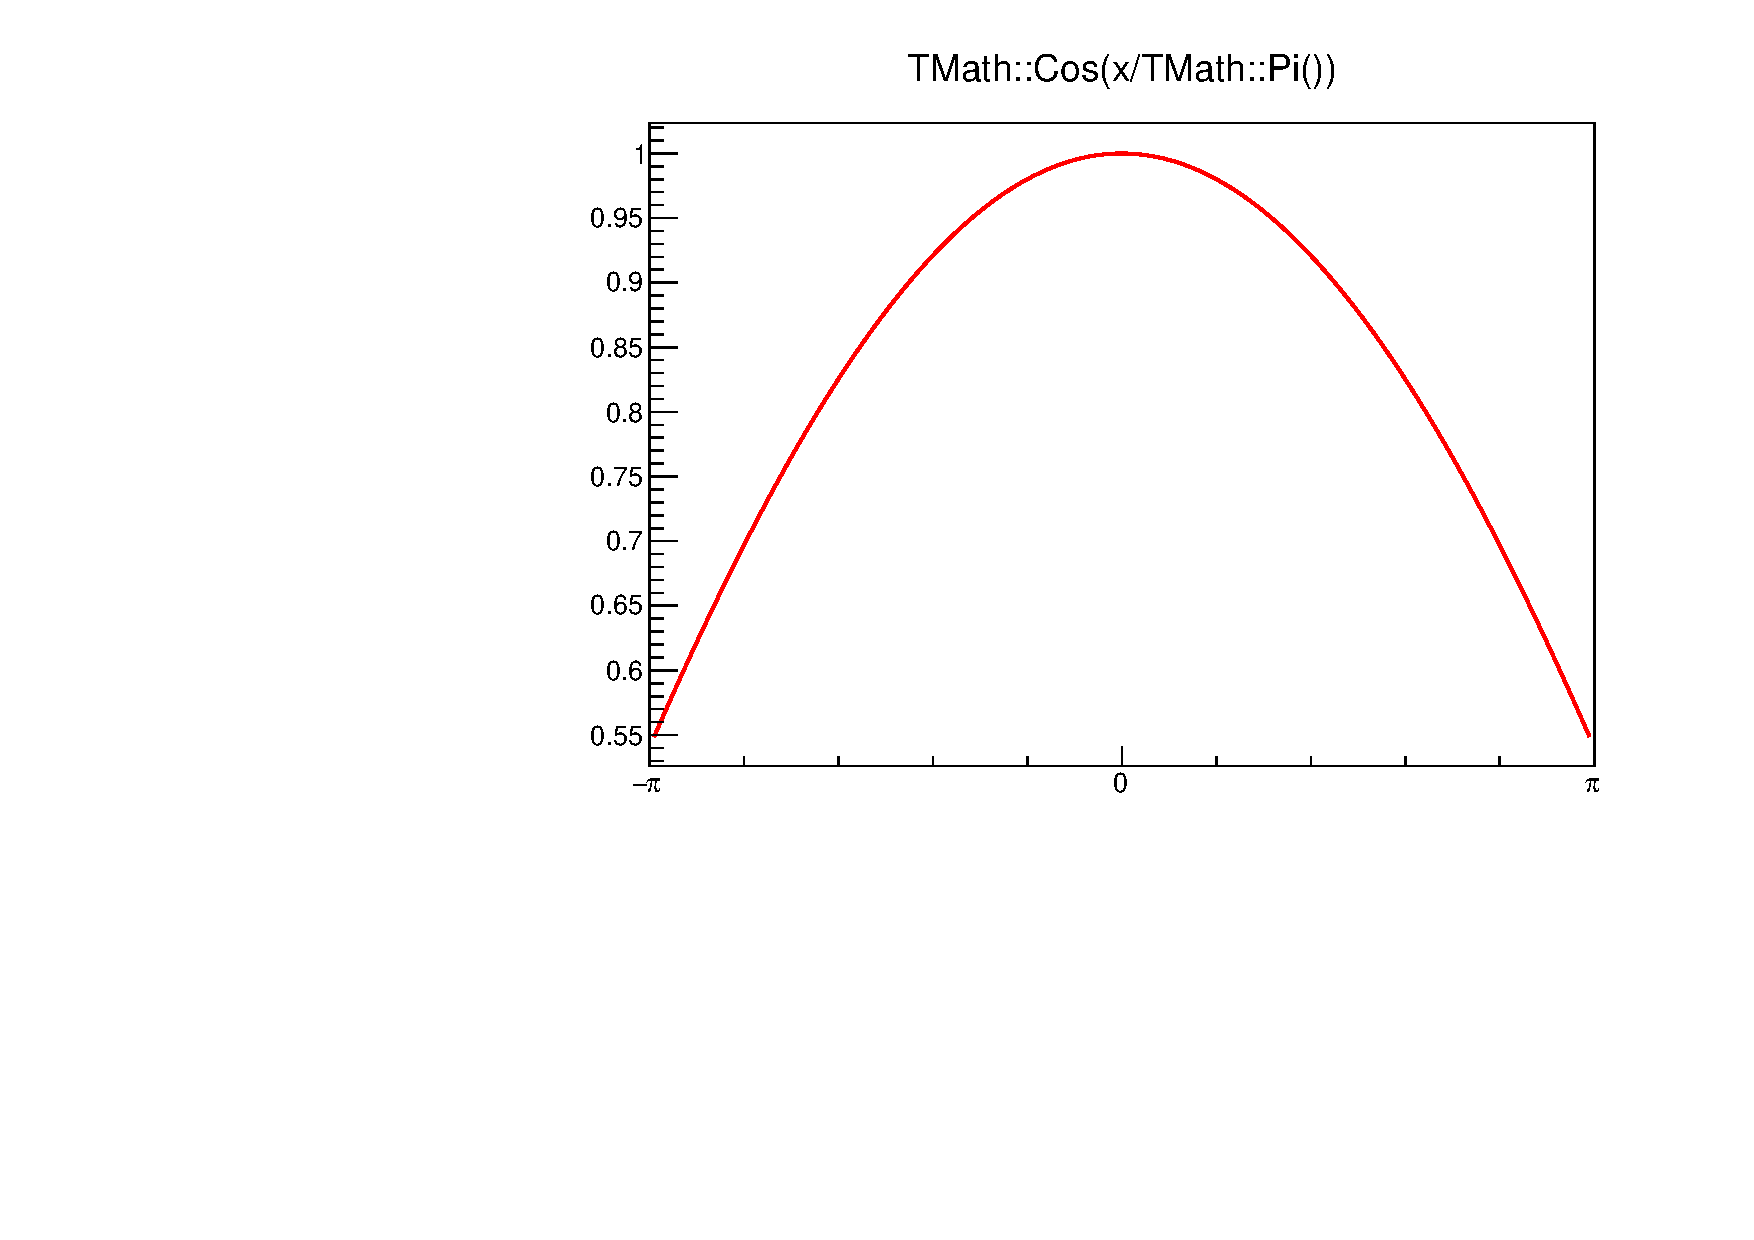
\includegraphics[width=0.7\linewidth]{assets/tgaxis.pdf}
  
\end{frame}

\section{User interactivity}

\begin{frame}[t]{Intercept and react to user interaction}
  \begin{itemize}
    \item \texttt{TRatioPlot} needs to know when content in the pads changes
    \item Use Signal/Slot mechanism to be called whenever interaction occurs
      \begin{itemize}
        \item Existing signal: \texttt{RangeAxisChanged}. Is emitted additionally in \texttt{TPad} on \texttt{SetLogx}, \texttt{SetLogy} and \texttt{SetLogz}
        \item New signal: \texttt{Resized} when pad is resized
        \item New signal: \texttt{UnZoomed} is called when the range of the axis is reset by the user
      \end{itemize}
    \item \texttt{TRatioPlot} connects to those signals
    \item Synchronizes pad margins, axes ranges, logx, and ensures the upper and lower pad meet at one point
    \item Inherits as many properties as possible from \texttt{gPad}
  \end{itemize}
\end{frame}

\section{Calculation modes}

\begin{frame}[t]{Available calculation and error modes}
  \begin{itemize}
    \item Divide two histograms using \texttt{TGraphAsymmErrors::Divide} (default, options given to \texttt{TRatioPlot} are passed through)
    \item Divide two histograms using \texttt{TH1::Divide}, yields symmetric errors (option \emph{divsym}, additional options are passed through)
    \item Subtract a histogram from another one (option \emph{diff})
    \item Subtract a histogram and divide by the uncertainty (option \emph{diffsig})
    \item Calculate residual between histogram and fitted function (invoked with corresponding constructor)
  \end{itemize}
  \uncover<2->{
  \begin{tabular}{p{2cm}|p{8cm}}
    Option & Error mode \\
    \hline
    errasym & Uses calculated asymmetric errors from \texttt{TH1::GetBinErrorUp}/\texttt{TH1::GetBinErrorLow}. Note that you need to set \texttt{TH1::SetBinErrorOption} first \\
    errfunc & Uses $\sqrt{f(x)}$ as the error \\
  \end{tabular}
  }
\end{frame}


\section{Examples}

\begin{frame}{\insertsection}
  \centering
  Ratio of two histograms
  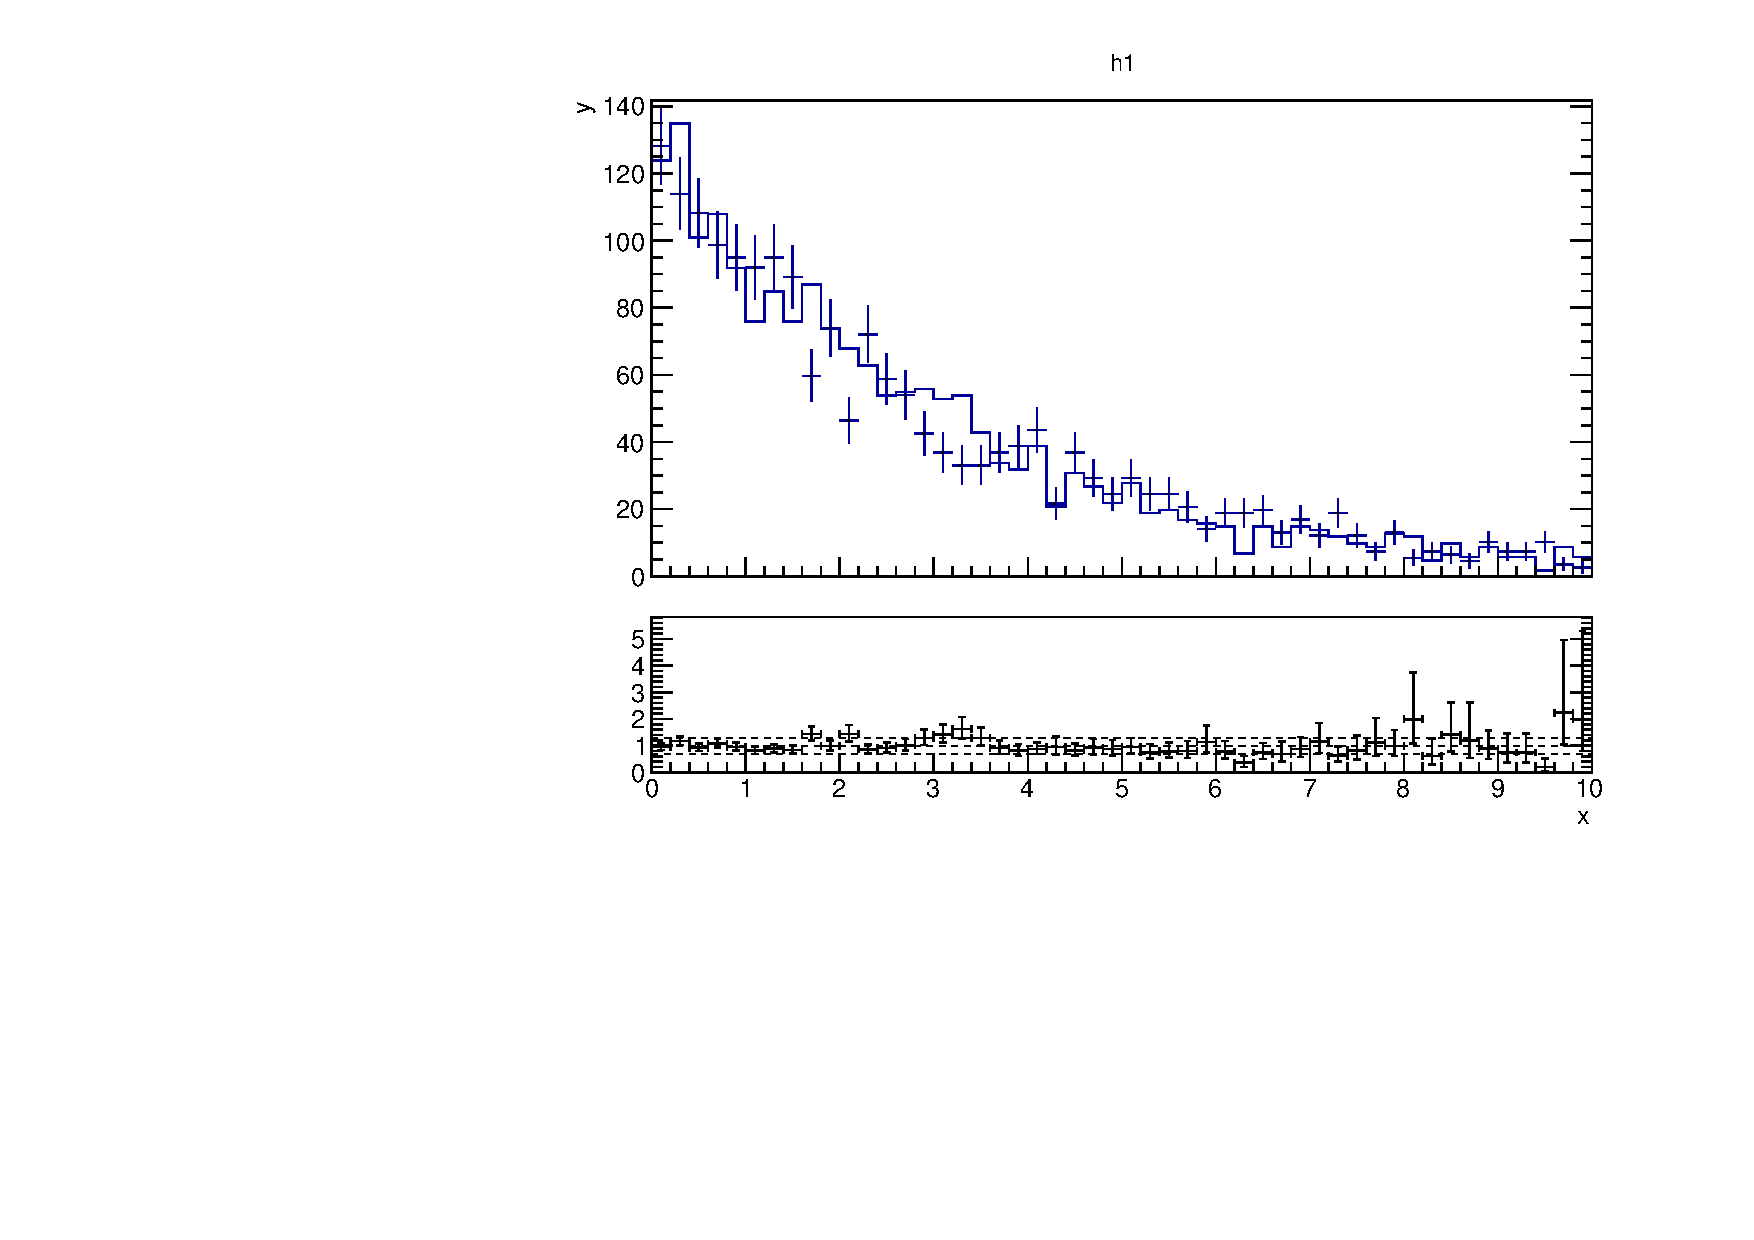
\includegraphics[width=0.9\linewidth]{assets/tut1.pdf} 
\end{frame}

\begin{frame}{\insertsection}
  \centering
  Difference between two histograms
  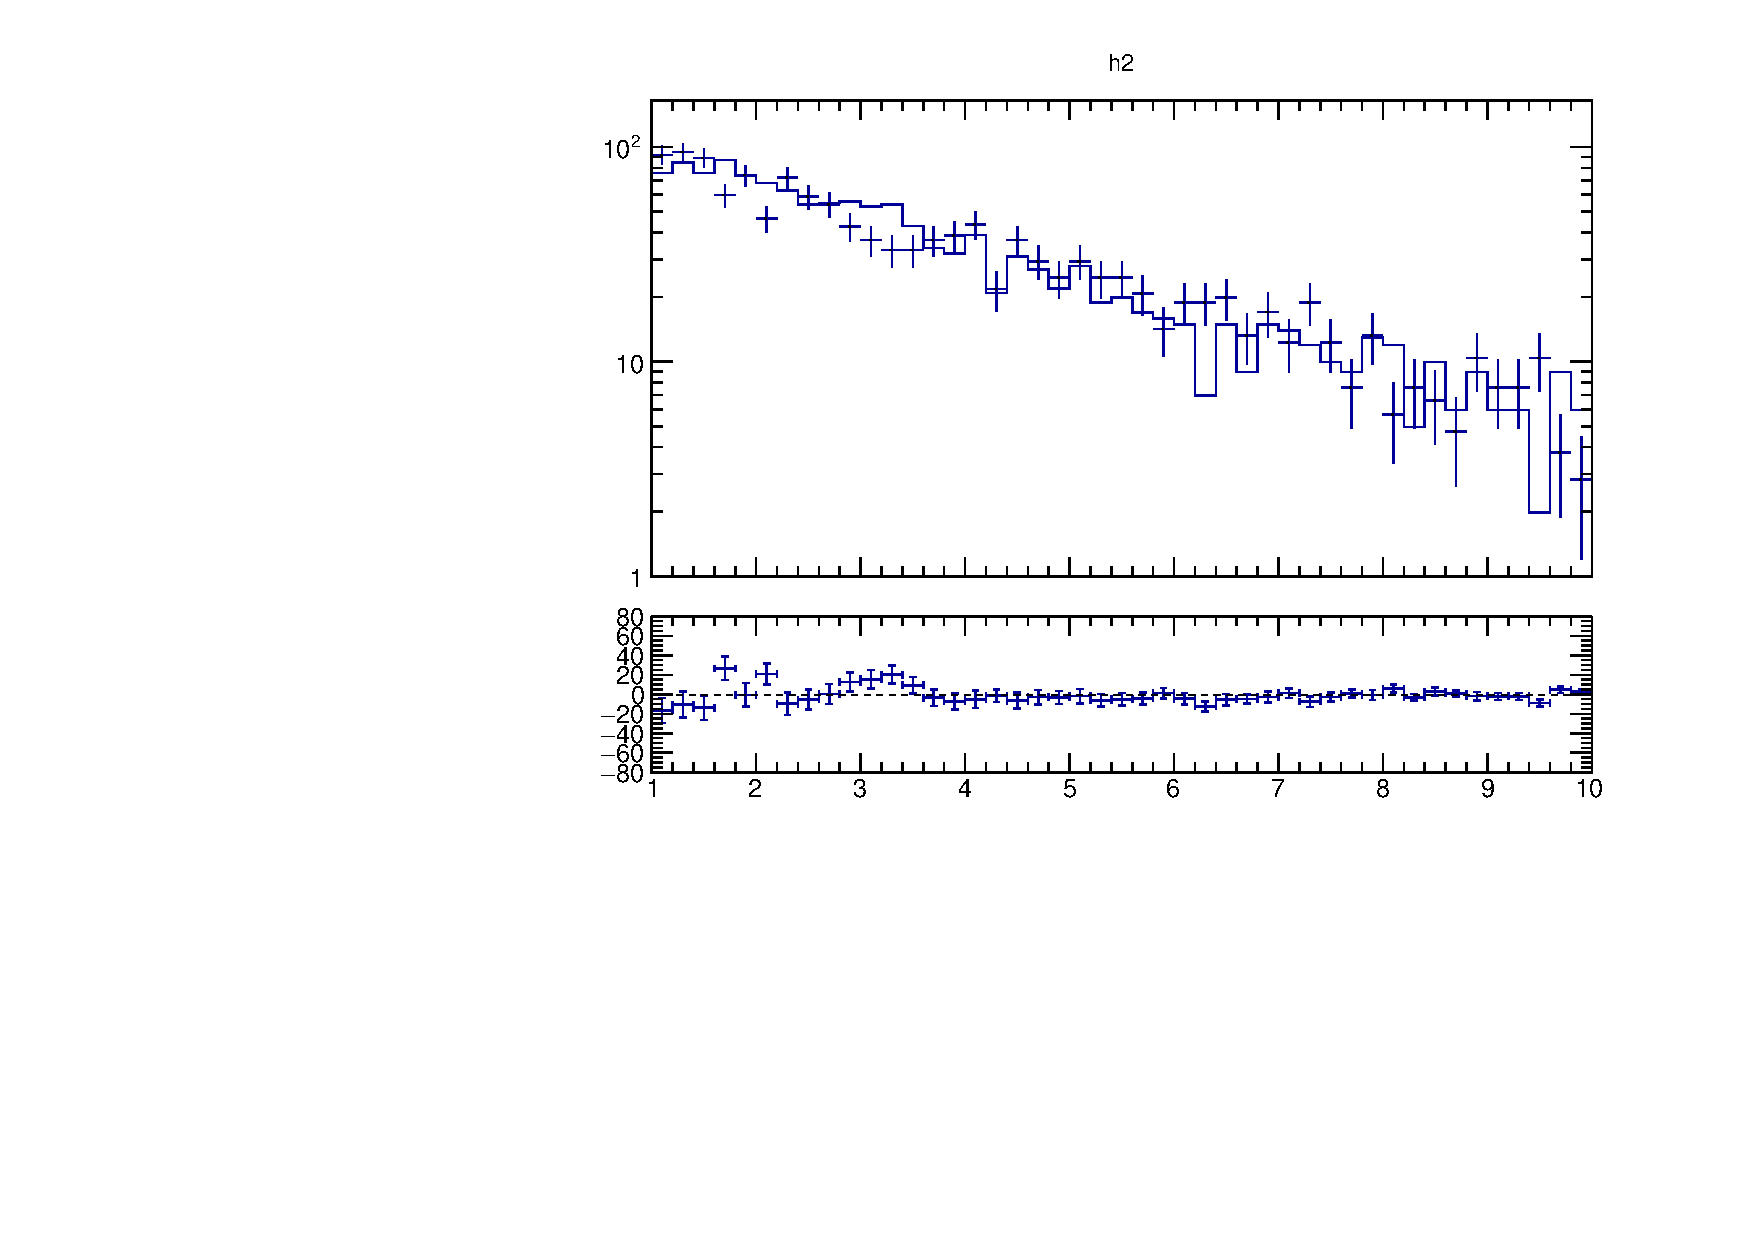
\includegraphics[width=0.9\linewidth]{assets/diff.pdf} 
\end{frame}

\begin{frame}{\insertsection}
  \centering
  Residual of histogram and a fit
  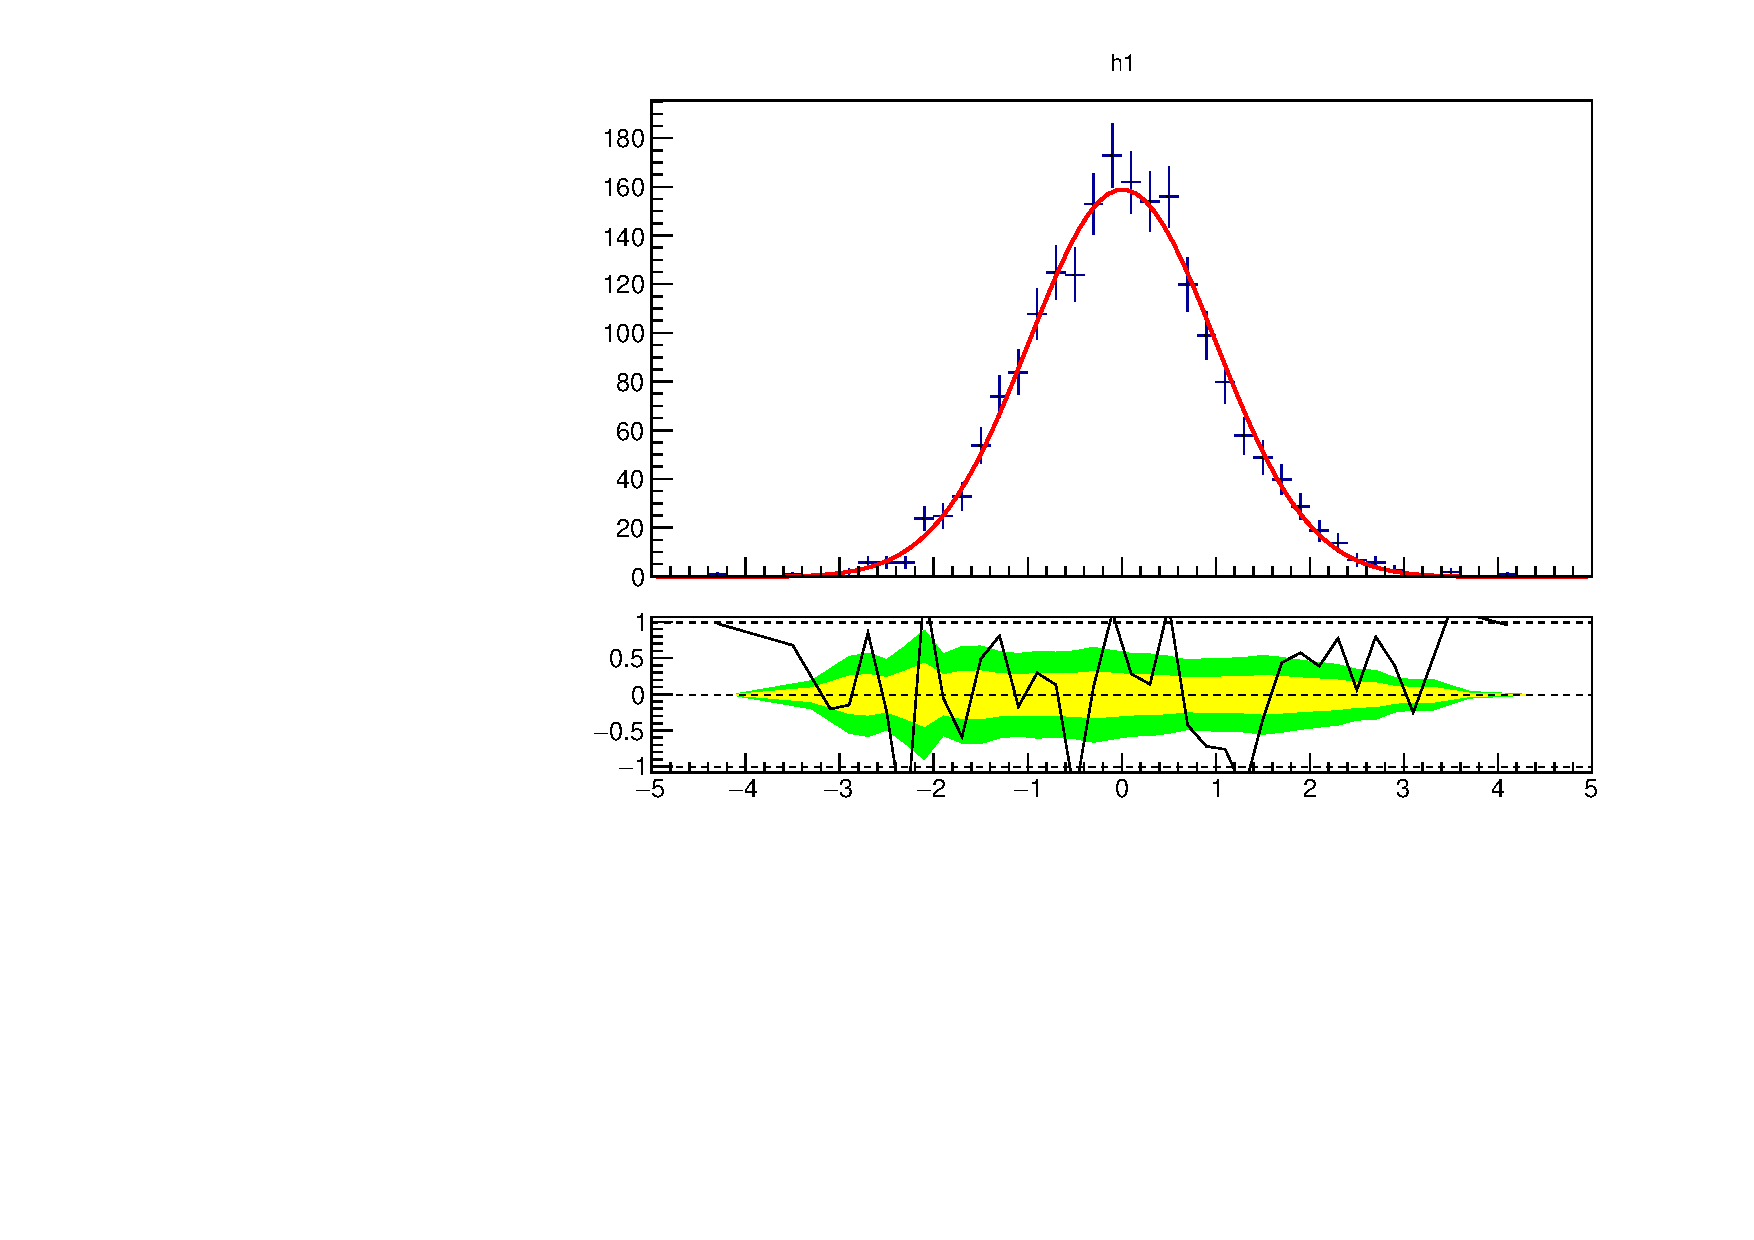
\includegraphics[width=0.9\linewidth]{assets/single.pdf} 
\end{frame}

\section{Programmatic usage}

\begin{frame}{Programmatic steering of display}
    \begin{itemize}
      \item In addition to interactivity, code duplication should be reduced
      \item Range and logx can be set on one pad and it is automatically synced
      \item Dashed lines can be customized by passing an array of y positions (\texttt{TRatioPlot::SetGridlines})
      \item Access to pads and all internals is provided with getters, so customization is possible
    \end{itemize}
    Necessary code to produce good looking results is reduced \bf{significantly}
\end{frame}

\begin{frame}[t]{Programmatic steering of display}
  \only<1>{
  Before: $\approx 50$ lines, $\approx 20$ lines of visual setup
  \tiny
  \lstinputlisting[language=C++]{assets/ratioplotOld.C}
  }
  \only<2>{
    With TRatioPlot: $\approx 20$ lines, $4$ lines of visual setup
  \tiny
  \lstinputlisting[language=C++]{assets/ratioplot1.C}
  }
\end{frame}

\begin{frame}[t]{Programmatic steering of display}
  \begin{columns}
    \column{0.5\linewidth}
    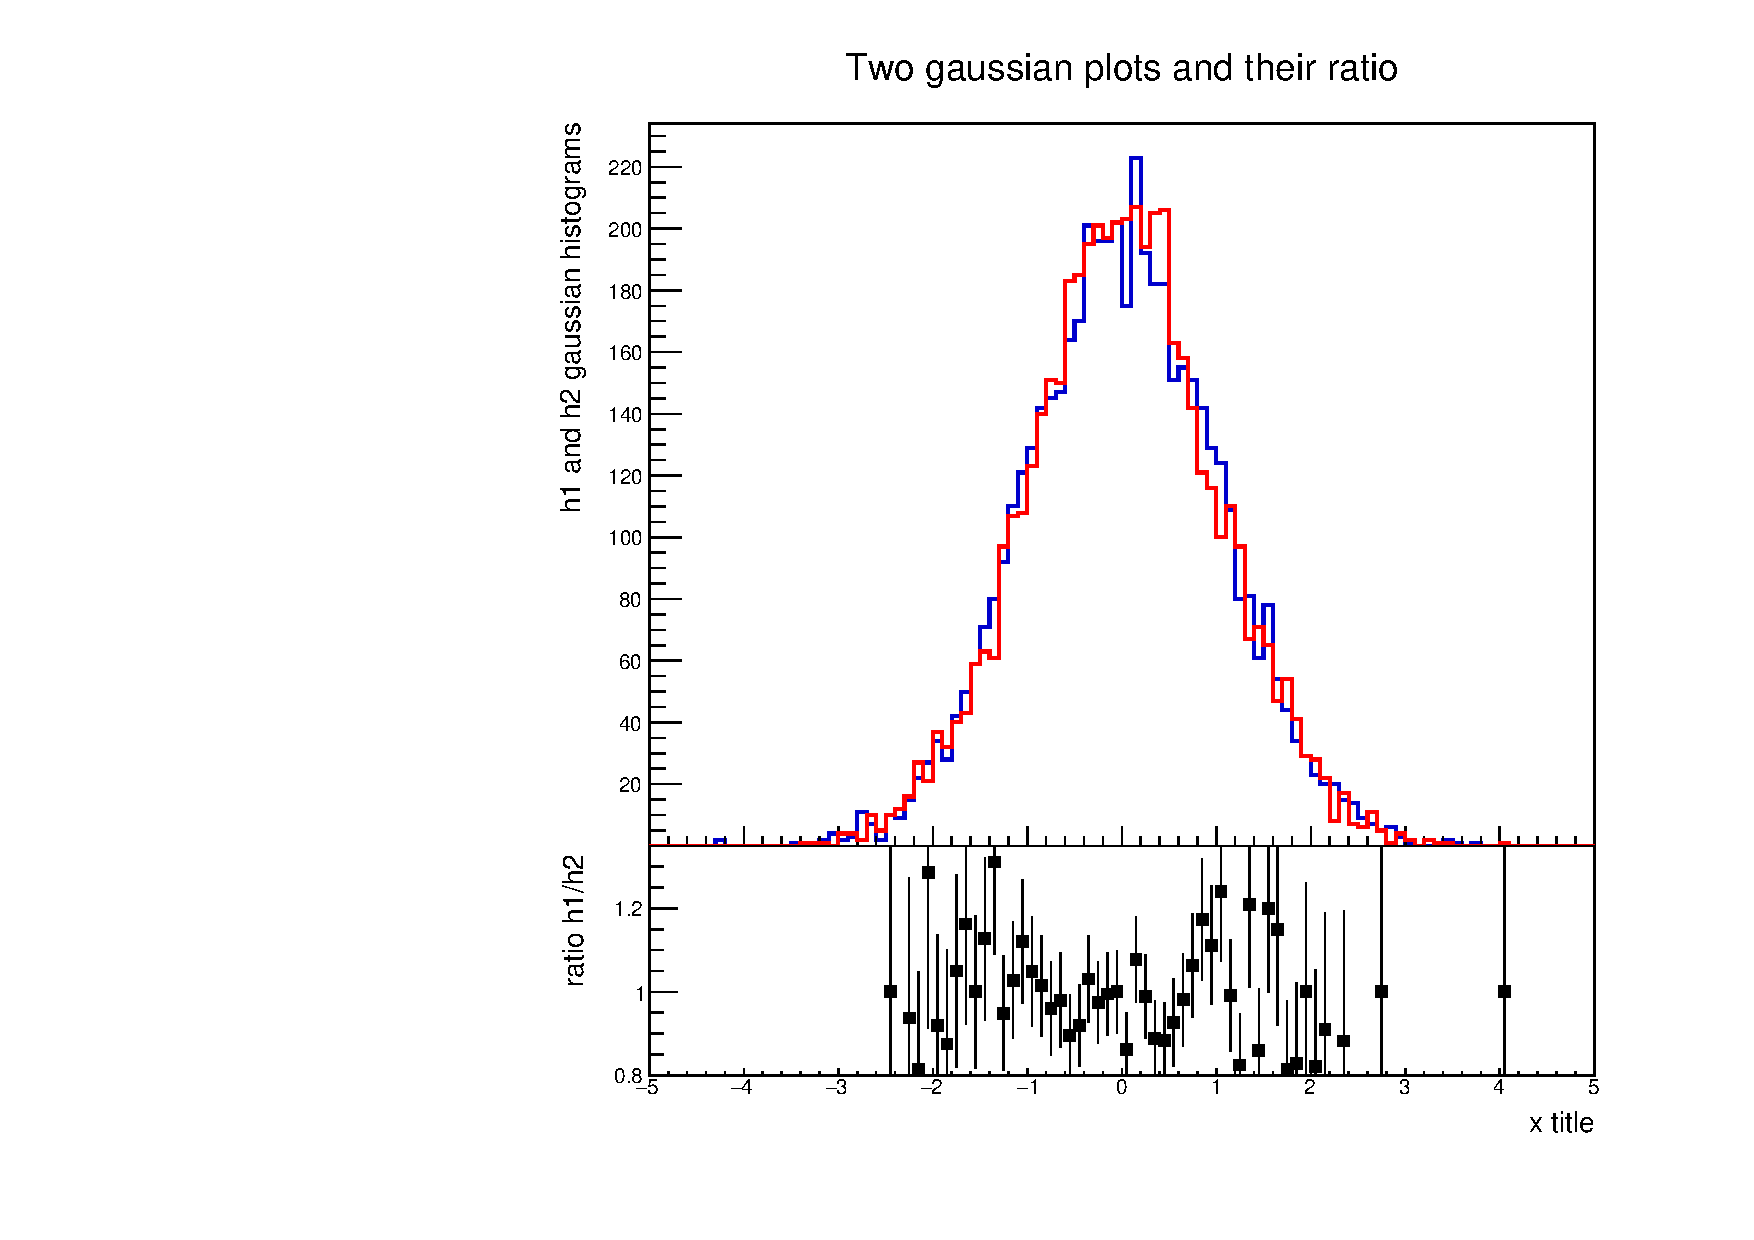
\includegraphics[width=1.0\linewidth]{assets/oldratio.pdf}
    \column{0.5\linewidth}
    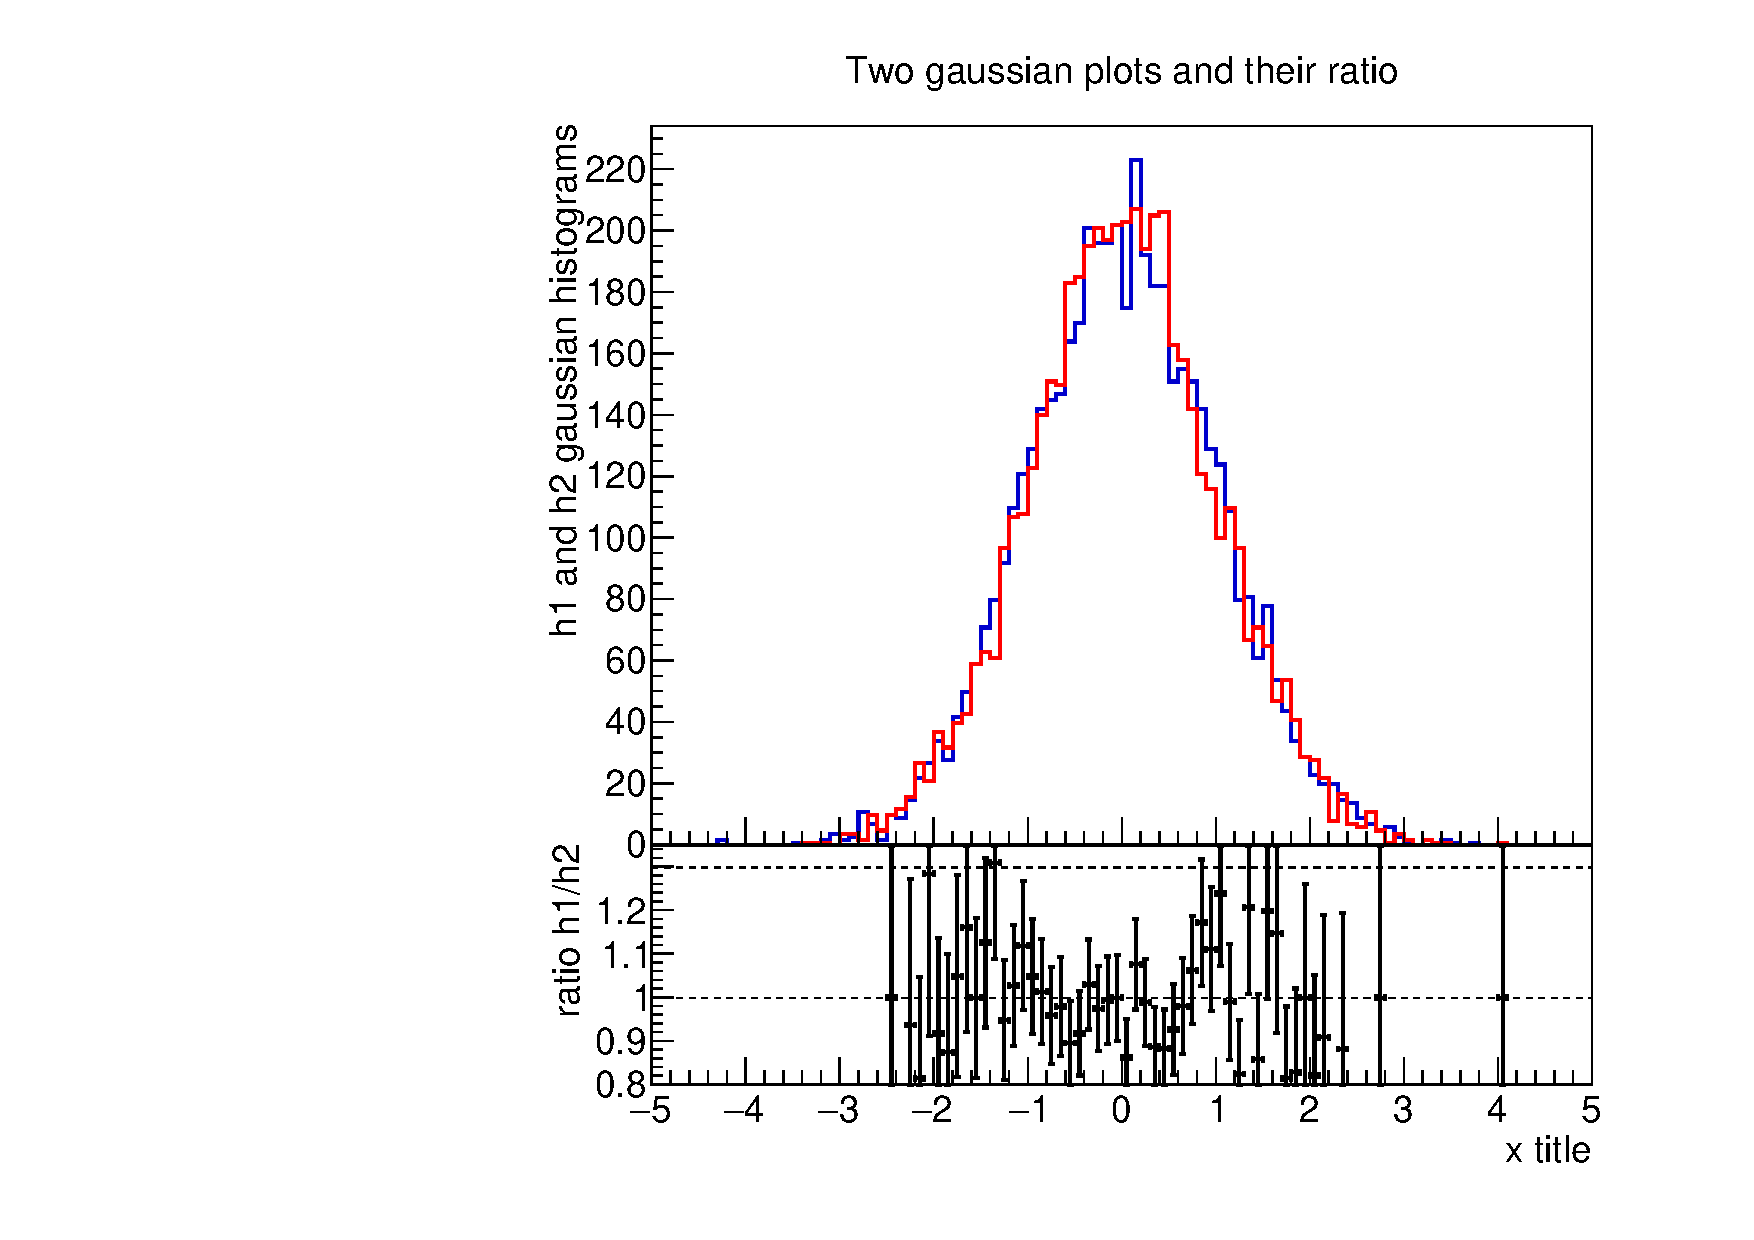
\includegraphics[width=1.0\linewidth]{assets/newratio.pdf}
  \end{columns}
\end{frame}

\begin{frame}[t]{Customization: ATLAS style}
  \only<1>{
  \centering
  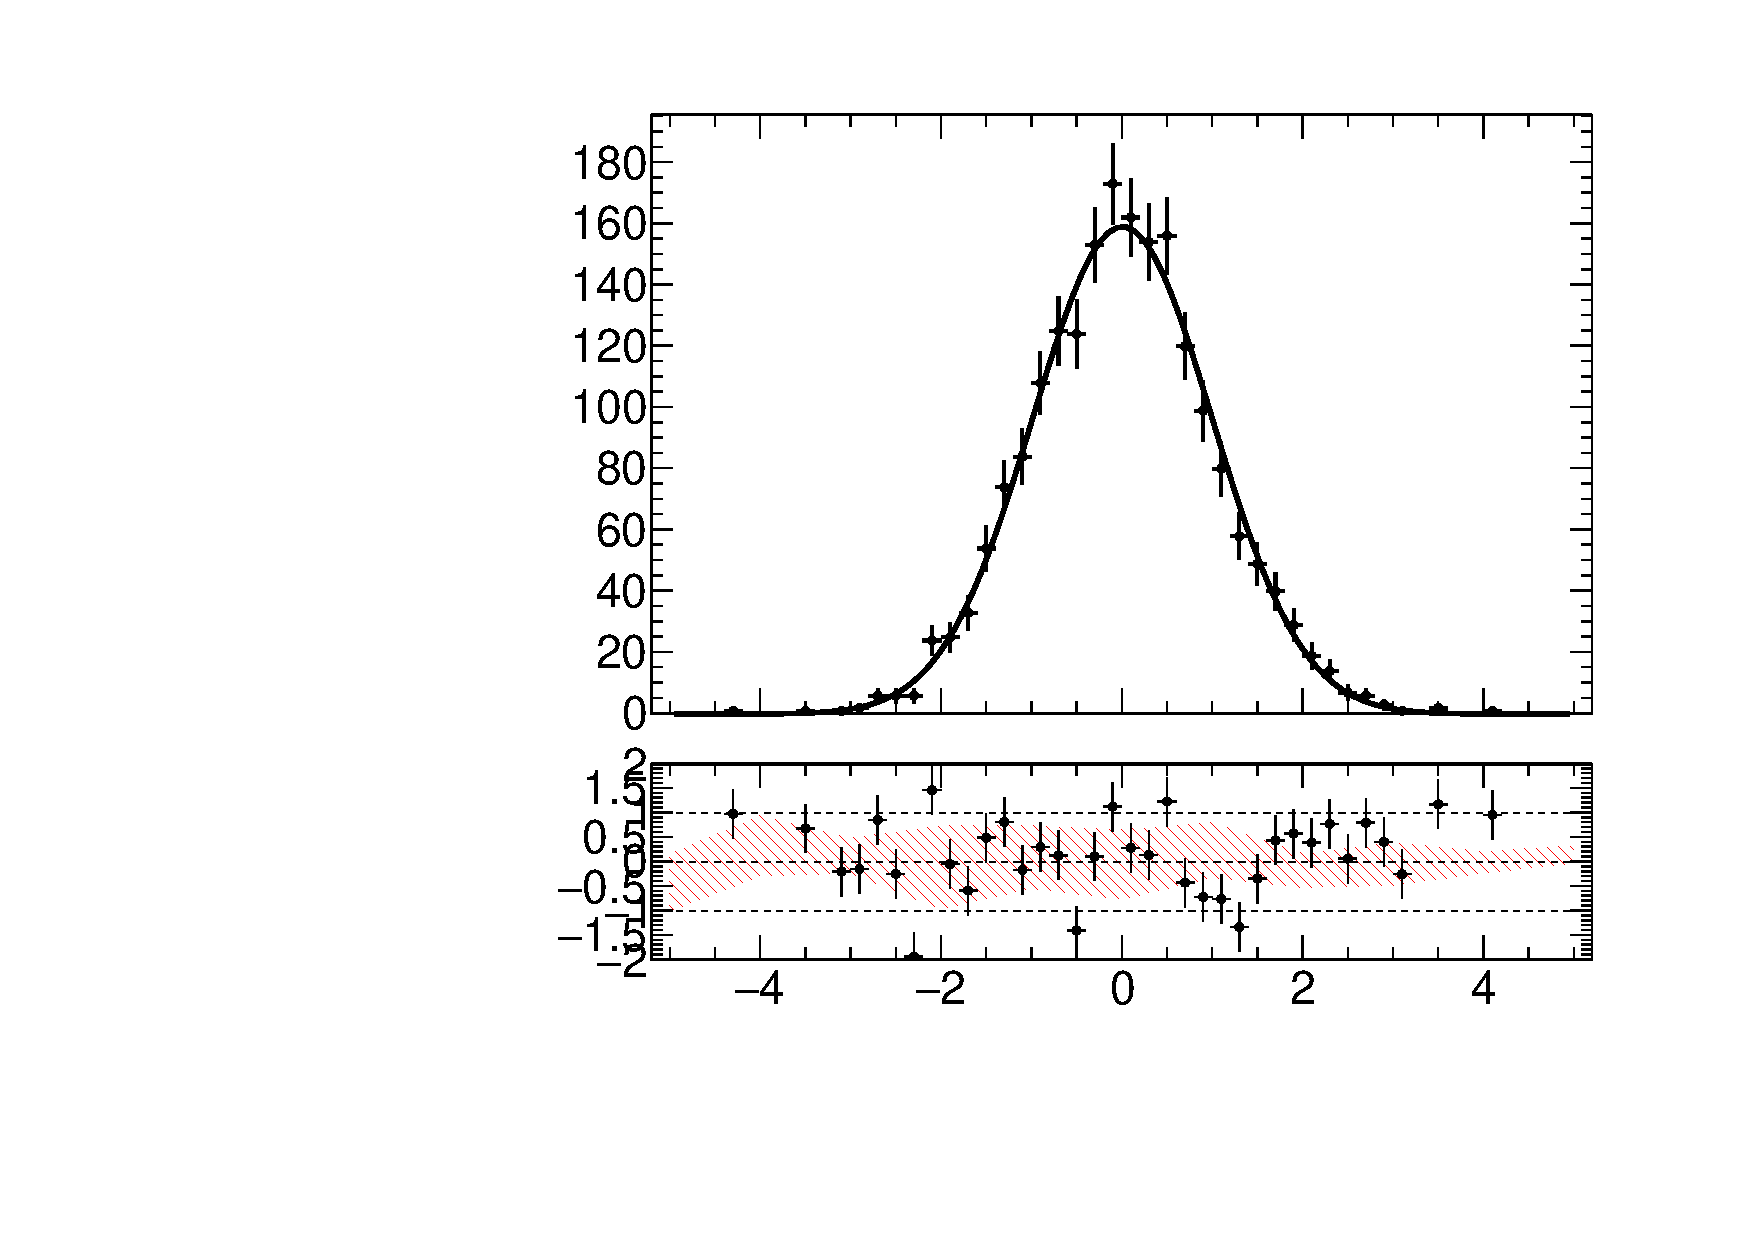
\includegraphics[width=0.8\linewidth]{assets/atlas.pdf}
  }
  \only<2>{
  \tiny
  \lstinputlisting[language=C++]{assets/atlas.C}
  }
\end{frame}

\begin{frame}[t]{Works with THStack out of the box}
  \only<1>{
  \centering
  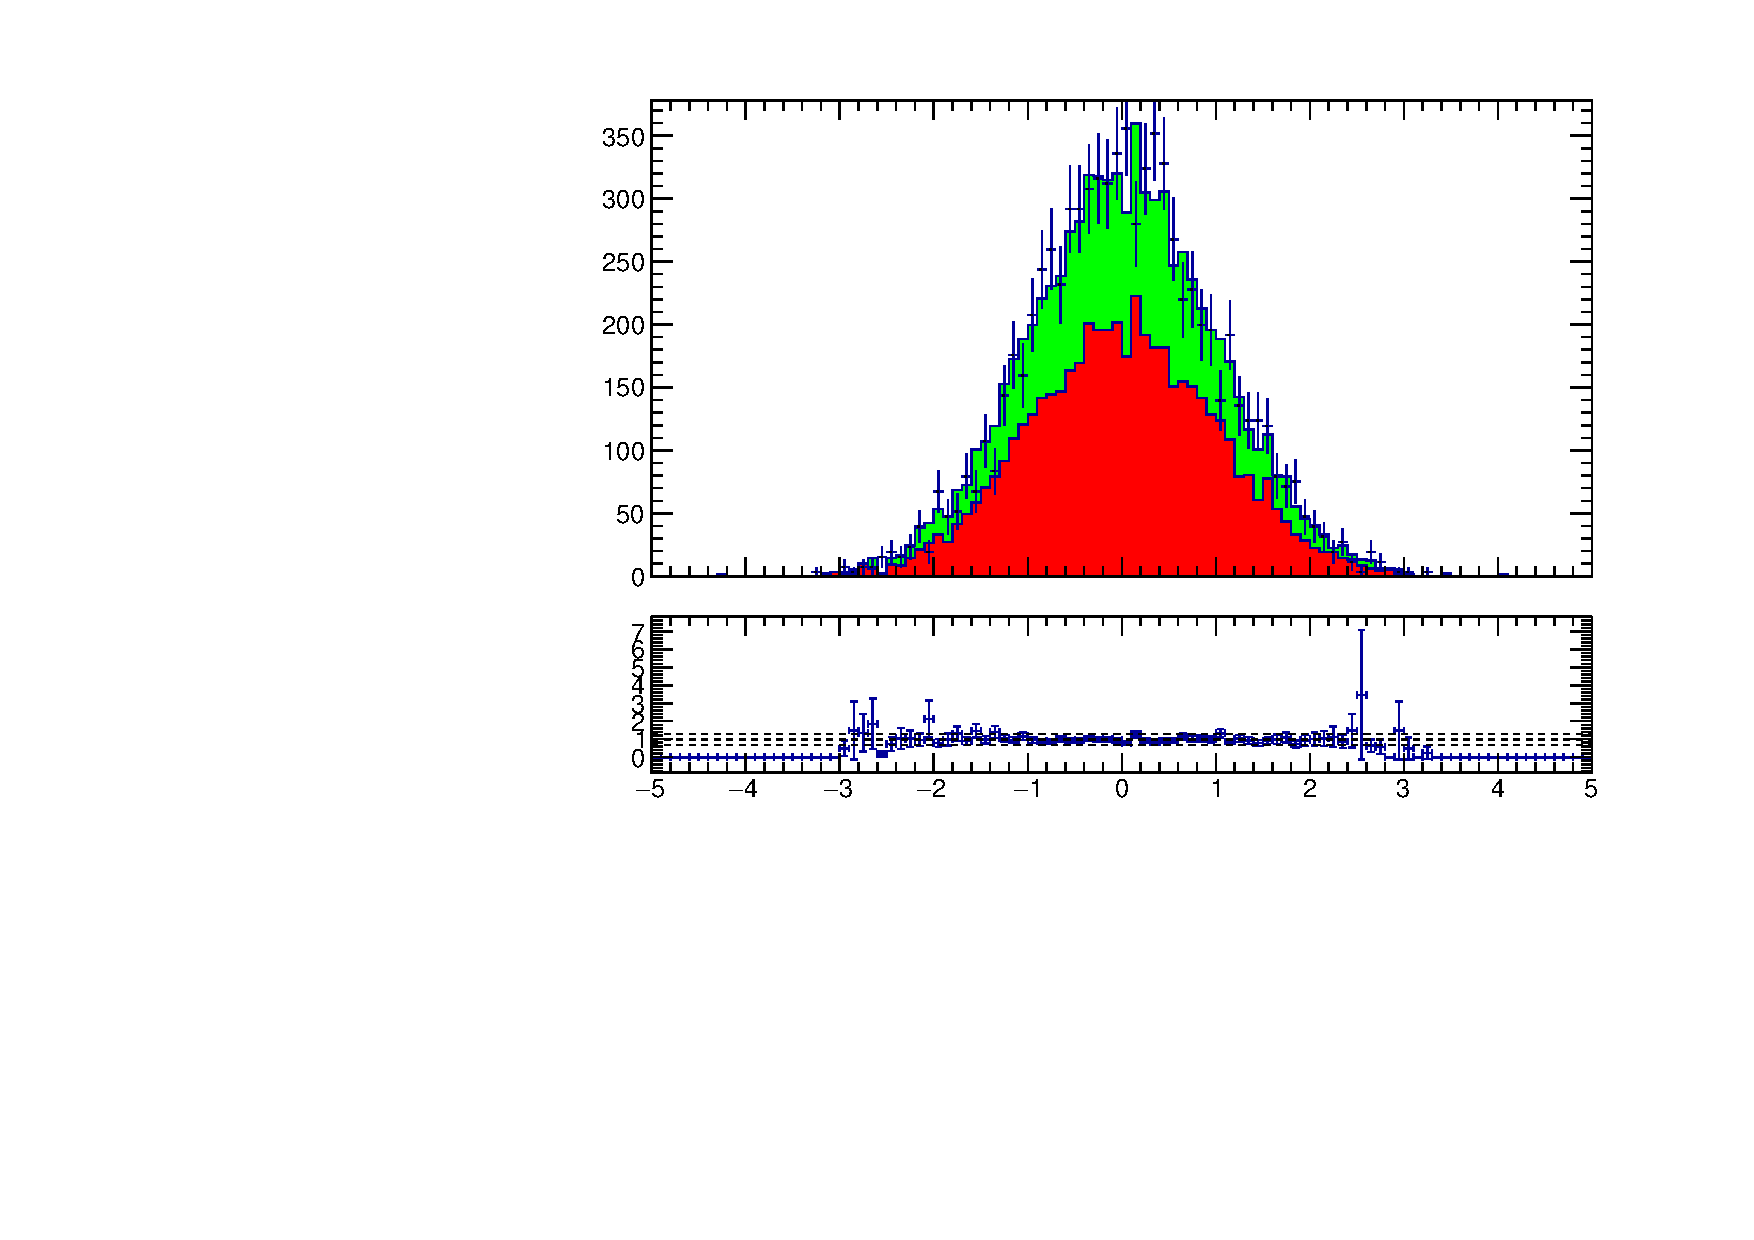
\includegraphics[width=0.9\linewidth]{assets/stack.pdf}
  }
  \only<2>{
  \tiny
  \lstinputlisting[language=C++]{assets/stack.C}
  }
\end{frame}

\begin{frame}[t]{Summary}
  Status:
  \begin{itemize}
    \item Class performing drawing and synchronization of two pads has been created
    \item Performs most common calculations
    \item Merged in master and ready to go
  \end{itemize}
  Possible improvements:
  \begin{itemize}
    \item Refresh of canvas is still an issue, artifacts appear and occasionally stick until manual window resize
      \begin{itemize}
        \item No problems observed in static case
      \end{itemize} 
    \item Only works with two pads
      \begin{itemize}
        \item Generalization to have mutliple pads linked together would be useful (tested on prototype)
        \item Calculation input would have to be flexible
      \end{itemize}
  \end{itemize}
\end{frame}

%\beg{Work in progress}
  %\begin{itemize}
    %\item Basic implementation working
    %\item Refinement in progress
    %\item Documentation is pending
    %\item Additional features:
      %\begin{itemize}
        %\item Automatic drawing of gridlines at 0, 1 depending on plot type
        %\item Automatic drawing of confidence bands for fit residual based on fit parameter uncertainties
      %\end{itemize}
    %\item Possible improvements:
      %\begin{itemize}
        %\item Generalization to more than two pads
      %\end{itemize}
  %\end{itemize}
%\end{frame}



\begin{frame}[allowframebreaks]{}
  \tiny{
  \printbibliography
  }
\end{frame}


\end{document}
